% Overview
\newcommand{\aSentencesAll}{2528}
\newcommand{\aSentencesI}{292}
\newcommand{\aSentencesII}{366}
\newcommand{\aSentencesIII}{320}
\newcommand{\aSentencesIV}{352}
\newcommand{\aSentencesV}{344}
\newcommand{\aSentencesVI}{289}
\newcommand{\aSentencesVII}{365}
\newcommand{\aSentencesVIII}{200}

\newcommand{\aWordsAll}{16187}
\newcommand{\aWordsI}{2089}
\newcommand{\aWordsII}{2162}
\newcommand{\aWordsIII}{2115}
\newcommand{\aWordsIV}{2035}
\newcommand{\aWordsV}{2217}
\newcommand{\aWordsVI}{2033}
\newcommand{\aWordsVII}{2322}
\newcommand{\aWordsVIII}{1214}

\newcommand{\aPhonesAll}{66611}
\newcommand{\aPhonesI}{8802}
\newcommand{\aPhonesII}{8727}
\newcommand{\aPhonesIII}{8770}
\newcommand{\aPhonesIV}{8557}
\newcommand{\aPhonesV}{9197}
\newcommand{\aPhonesVI}{8353}
\newcommand{\aPhonesVII}{9351}
\newcommand{\aPhonesVIII}{4854}


% Sentences by Speaker
\newcommand{\aBubbaAll}{74}
\newcommand{\aBubbaI}{0}
\newcommand{\aBubbaII}{16}
\newcommand{\aBubbaIII}{40}
\newcommand{\aBubbaIV}{18}
\newcommand{\aBubbaV}{0}
\newcommand{\aBubbaVI}{0}
\newcommand{\aBubbaVII}{0}
\newcommand{\aBubbaVIII}{0}

\newcommand{\aForrestAll}{354}
\newcommand{\aForrestI}{22}
\newcommand{\aForrestII}{37}
\newcommand{\aForrestIII}{22}
\newcommand{\aForrestIV}{48}
\newcommand{\aForrestV}{50}
\newcommand{\aForrestVI}{61}
\newcommand{\aForrestVII}{49}
\newcommand{\aForrestVIII}{65}

\newcommand{\aForrestchildAll}{19}
\newcommand{\aForrestchildI}{17}
\newcommand{\aForrestchildII}{2}
\newcommand{\aForrestchildIII}{0}
\newcommand{\aForrestchildIV}{0}
\newcommand{\aForrestchildV}{0}
\newcommand{\aForrestchildVI}{0}
\newcommand{\aForrestchildVII}{0}
\newcommand{\aForrestchildVIII}{0}

\newcommand{\aForrestvoAll}{369}
\newcommand{\aForrestvoI}{61}
\newcommand{\aForrestvoII}{48}
\newcommand{\aForrestvoIII}{53}
\newcommand{\aForrestvoIV}{51}
\newcommand{\aForrestvoV}{37}
\newcommand{\aForrestvoVI}{40}
\newcommand{\aForrestvoVII}{63}
\newcommand{\aForrestvoVIII}{16}

\newcommand{\aHancockAll}{16}
\newcommand{\aHancockI}{16}
\newcommand{\aHancockII}{0}
\newcommand{\aHancockIII}{0}
\newcommand{\aHancockIV}{0}
\newcommand{\aHancockV}{0}
\newcommand{\aHancockVI}{0}
\newcommand{\aHancockVII}{0}
\newcommand{\aHancockVIII}{0}

\newcommand{\aJennyAll}{177}
\newcommand{\aJennyI}{0}
\newcommand{\aJennyII}{46}
\newcommand{\aJennyIII}{30}
\newcommand{\aJennyIV}{3}
\newcommand{\aJennyV}{25}
\newcommand{\aJennyVI}{0}
\newcommand{\aJennyVII}{57}
\newcommand{\aJennyVIII}{16}

\newcommand{\aJennychildAll}{23}
\newcommand{\aJennychildI}{7}
\newcommand{\aJennychildII}{16}
\newcommand{\aJennychildIII}{0}
\newcommand{\aJennychildIV}{0}
\newcommand{\aJennychildV}{0}
\newcommand{\aJennychildVI}{0}
\newcommand{\aJennychildVII}{0}
\newcommand{\aJennychildVIII}{0}

\newcommand{\aLtdanAll}{183}
\newcommand{\aLtdanI}{0}
\newcommand{\aLtdanII}{0}
\newcommand{\aLtdanIII}{49}
\newcommand{\aLtdanIV}{33}
\newcommand{\aLtdanV}{65}
\newcommand{\aLtdanVI}{28}
\newcommand{\aLtdanVII}{0}
\newcommand{\aLtdanVIII}{8}

\newcommand{\aMrsgumpAll}{53}
\newcommand{\aMrsgumpI}{38}
\newcommand{\aMrsgumpII}{2}
\newcommand{\aMrsgumpIII}{0}
\newcommand{\aMrsgumpIV}{0}
\newcommand{\aMrsgumpV}{0}
\newcommand{\aMrsgumpVI}{13}
\newcommand{\aMrsgumpVII}{0}
\newcommand{\aMrsgumpVIII}{0}

\newcommand{\aNarratorAll}{903}
\newcommand{\aNarratorI}{111}
\newcommand{\aNarratorII}{134}
\newcommand{\aNarratorIII}{78}
\newcommand{\aNarratorIV}{139}
\newcommand{\aNarratorV}{93}
\newcommand{\aNarratorVI}{115}
\newcommand{\aNarratorVII}{147}
\newcommand{\aNarratorVIII}{86}


% POS-Tagging
\newcommand{\aPosAdj}{adjective}
\newcommand{\aPosAdjAll}{916}
\newcommand{\aPosAdjI}{138}
\newcommand{\aPosAdjII}{126}
\newcommand{\aPosAdjIII}{106}
\newcommand{\aPosAdjIV}{96}
\newcommand{\aPosAdjV}{130}
\newcommand{\aPosAdjVI}{118}
\newcommand{\aPosAdjVII}{128}
\newcommand{\aPosAdjVIII}{74}

\newcommand{\aPosAdp}{adposition}
\newcommand{\aPosAdpAll}{1429}
\newcommand{\aPosAdpI}{181}
\newcommand{\aPosAdpII}{176}
\newcommand{\aPosAdpIII}{176}
\newcommand{\aPosAdpIV}{194}
\newcommand{\aPosAdpV}{188}
\newcommand{\aPosAdpVI}{183}
\newcommand{\aPosAdpVII}{213}
\newcommand{\aPosAdpVIII}{118}

\newcommand{\aPosAdv}{adverb}
\newcommand{\aPosAdvAll}{1332}
\newcommand{\aPosAdvI}{166}
\newcommand{\aPosAdvII}{169}
\newcommand{\aPosAdvIII}{220}
\newcommand{\aPosAdvIV}{162}
\newcommand{\aPosAdvV}{178}
\newcommand{\aPosAdvVI}{169}
\newcommand{\aPosAdvVII}{193}
\newcommand{\aPosAdvVIII}{75}

\newcommand{\aPosAux}{auxiliary}
\newcommand{\aPosAuxAll}{807}
\newcommand{\aPosAuxI}{102}
\newcommand{\aPosAuxII}{120}
\newcommand{\aPosAuxIII}{92}
\newcommand{\aPosAuxIV}{96}
\newcommand{\aPosAuxV}{125}
\newcommand{\aPosAuxVI}{110}
\newcommand{\aPosAuxVII}{112}
\newcommand{\aPosAuxVIII}{50}

\newcommand{\aPosConj}{conjunction}
\newcommand{\aPosConjAll}{525}
\newcommand{\aPosConjI}{74}
\newcommand{\aPosConjII}{63}
\newcommand{\aPosConjIII}{71}
\newcommand{\aPosConjIV}{49}
\newcommand{\aPosConjV}{61}
\newcommand{\aPosConjVI}{80}
\newcommand{\aPosConjVII}{86}
\newcommand{\aPosConjVIII}{41}

\newcommand{\aPosDet}{determiner}
\newcommand{\aPosDetAll}{1754}
\newcommand{\aPosDetI}{257}
\newcommand{\aPosDetII}{243}
\newcommand{\aPosDetIII}{198}
\newcommand{\aPosDetIV}{219}
\newcommand{\aPosDetV}{220}
\newcommand{\aPosDetVI}{222}
\newcommand{\aPosDetVII}{254}
\newcommand{\aPosDetVIII}{141}

\newcommand{\aPosNonspeechAll}{202}
\newcommand{\aPosNonspeechI}{23}
\newcommand{\aPosNonspeechII}{21}
\newcommand{\aPosNonspeechIII}{9}
\newcommand{\aPosNonspeechIV}{23}
\newcommand{\aPosNonspeechV}{55}
\newcommand{\aPosNonspeechVI}{44}
\newcommand{\aPosNonspeechVII}{13}
\newcommand{\aPosNonspeechVIII}{14}

\newcommand{\aPosNoun}{noun}
\newcommand{\aPosNounAll}{2620}
\newcommand{\aPosNounI}{361}
\newcommand{\aPosNounII}{341}
\newcommand{\aPosNounIII}{332}
\newcommand{\aPosNounIV}{343}
\newcommand{\aPosNounV}{331}
\newcommand{\aPosNounVI}{356}
\newcommand{\aPosNounVII}{351}
\newcommand{\aPosNounVIII}{205}

\newcommand{\aPosNum}{numeral}
\newcommand{\aPosNumAll}{66}
\newcommand{\aPosNumI}{8}
\newcommand{\aPosNumII}{11}
\newcommand{\aPosNumIII}{11}
\newcommand{\aPosNumIV}{7}
\newcommand{\aPosNumV}{4}
\newcommand{\aPosNumVI}{9}
\newcommand{\aPosNumVII}{14}
\newcommand{\aPosNumVIII}{2}

\newcommand{\aPosPart}{particle}
\newcommand{\aPosPartAll}{572}
\newcommand{\aPosPartI}{60}
\newcommand{\aPosPartII}{100}
\newcommand{\aPosPartIII}{90}
\newcommand{\aPosPartIV}{62}
\newcommand{\aPosPartV}{83}
\newcommand{\aPosPartVI}{53}
\newcommand{\aPosPartVII}{86}
\newcommand{\aPosPartVIII}{38}

\newcommand{\aPosPron}{pronoun}
\newcommand{\aPosPronAll}{2348}
\newcommand{\aPosPronI}{275}
\newcommand{\aPosPronII}{321}
\newcommand{\aPosPronIII}{328}
\newcommand{\aPosPronIV}{260}
\newcommand{\aPosPronV}{348}
\newcommand{\aPosPronVI}{262}
\newcommand{\aPosPronVII}{362}
\newcommand{\aPosPronVIII}{192}

\newcommand{\aPosPropn}{proper noun}
\newcommand{\aPosPropnAll}{1012}
\newcommand{\aPosPropnI}{131}
\newcommand{\aPosPropnII}{135}
\newcommand{\aPosPropnIII}{119}
\newcommand{\aPosPropnIV}{168}
\newcommand{\aPosPropnV}{162}
\newcommand{\aPosPropnVI}{116}
\newcommand{\aPosPropnVII}{117}
\newcommand{\aPosPropnVIII}{64}

\newcommand{\aPosSconj}{subordinating conjunction}
\newcommand{\aPosSconjAll}{172}
\newcommand{\aPosSconjI}{19}
\newcommand{\aPosSconjII}{18}
\newcommand{\aPosSconjIII}{20}
\newcommand{\aPosSconjIV}{15}
\newcommand{\aPosSconjV}{31}
\newcommand{\aPosSconjVI}{27}
\newcommand{\aPosSconjVII}{26}
\newcommand{\aPosSconjVIII}{16}

\newcommand{\aPosVerb}{verb}
\newcommand{\aPosVerbAll}{2317}
\newcommand{\aPosVerbI}{285}
\newcommand{\aPosVerbII}{308}
\newcommand{\aPosVerbIII}{320}
\newcommand{\aPosVerbIV}{319}
\newcommand{\aPosVerbV}{289}
\newcommand{\aPosVerbVI}{274}
\newcommand{\aPosVerbVII}{349}
\newcommand{\aPosVerbVIII}{173}

\newcommand{\aPosX}{other}
\newcommand{\aPosXAll}{108}
\newcommand{\aPosXI}{8}
\newcommand{\aPosXII}{10}
\newcommand{\aPosXIII}{21}
\newcommand{\aPosXIV}{21}
\newcommand{\aPosXV}{11}
\newcommand{\aPosXVI}{9}
\newcommand{\aPosXVII}{17}
\newcommand{\aPosXVIII}{11}


% TAG-Tagging
\newcommand{\aTagAdja}{adjective, attributive}
\newcommand{\aTagAdjaAll}{478}
\newcommand{\aTagAdjaI}{73}
\newcommand{\aTagAdjaII}{58}
\newcommand{\aTagAdjaIII}{58}
\newcommand{\aTagAdjaIV}{51}
\newcommand{\aTagAdjaV}{77}
\newcommand{\aTagAdjaVI}{58}
\newcommand{\aTagAdjaVII}{70}
\newcommand{\aTagAdjaVIII}{33}

\newcommand{\aTagAdjd}{adjective, adverbial or predicative}
\newcommand{\aTagAdjdAll}{438}
\newcommand{\aTagAdjdI}{65}
\newcommand{\aTagAdjdII}{68}
\newcommand{\aTagAdjdIII}{48}
\newcommand{\aTagAdjdIV}{45}
\newcommand{\aTagAdjdV}{53}
\newcommand{\aTagAdjdVI}{60}
\newcommand{\aTagAdjdVII}{58}
\newcommand{\aTagAdjdVIII}{41}

\newcommand{\aTagAdv}{adverb}
\newcommand{\aTagAdvAll}{1181}
\newcommand{\aTagAdvI}{146}
\newcommand{\aTagAdvII}{145}
\newcommand{\aTagAdvIII}{201}
\newcommand{\aTagAdvIV}{143}
\newcommand{\aTagAdvV}{157}
\newcommand{\aTagAdvVI}{149}
\newcommand{\aTagAdvVII}{174}
\newcommand{\aTagAdvVIII}{66}

\newcommand{\aTagAppr}{preposition; circumposition left}
\newcommand{\aTagApprAll}{1192}
\newcommand{\aTagApprI}{156}
\newcommand{\aTagApprII}{146}
\newcommand{\aTagApprIII}{156}
\newcommand{\aTagApprIV}{152}
\newcommand{\aTagApprV}{157}
\newcommand{\aTagApprVI}{150}
\newcommand{\aTagApprVII}{178}
\newcommand{\aTagApprVIII}{97}

\newcommand{\aTagArt}{definite or indefinite article}
\newcommand{\aTagArtAll}{1340}
\newcommand{\aTagArtI}{199}
\newcommand{\aTagArtII}{183}
\newcommand{\aTagArtIII}{140}
\newcommand{\aTagArtIV}{178}
\newcommand{\aTagArtV}{159}
\newcommand{\aTagArtVI}{176}
\newcommand{\aTagArtVII}{191}
\newcommand{\aTagArtVIII}{114}

\newcommand{\aTagKon}{coordinate conjunction}
\newcommand{\aTagKonAll}{475}
\newcommand{\aTagKonI}{58}
\newcommand{\aTagKonII}{58}
\newcommand{\aTagKonIII}{66}
\newcommand{\aTagKonIV}{45}
\newcommand{\aTagKonV}{58}
\newcommand{\aTagKonVI}{76}
\newcommand{\aTagKonVII}{78}
\newcommand{\aTagKonVIII}{36}

\newcommand{\aTagNe}{proper noun}
\newcommand{\aTagNeAll}{1012}
\newcommand{\aTagNeI}{131}
\newcommand{\aTagNeII}{135}
\newcommand{\aTagNeIII}{119}
\newcommand{\aTagNeIV}{168}
\newcommand{\aTagNeV}{162}
\newcommand{\aTagNeVI}{116}
\newcommand{\aTagNeVII}{117}
\newcommand{\aTagNeVIII}{64}

\newcommand{\aTagNn}{noun, singular or mass}
\newcommand{\aTagNnAll}{2620}
\newcommand{\aTagNnI}{361}
\newcommand{\aTagNnII}{341}
\newcommand{\aTagNnIII}{332}
\newcommand{\aTagNnIV}{343}
\newcommand{\aTagNnV}{331}
\newcommand{\aTagNnVI}{356}
\newcommand{\aTagNnVII}{351}
\newcommand{\aTagNnVIII}{205}

\newcommand{\aTagPper}{non-reflexive personal pronoun}
\newcommand{\aTagPperAll}{1638}
\newcommand{\aTagPperI}{183}
\newcommand{\aTagPperII}{210}
\newcommand{\aTagPperIII}{221}
\newcommand{\aTagPperIV}{168}
\newcommand{\aTagPperV}{246}
\newcommand{\aTagPperVI}{176}
\newcommand{\aTagPperVII}{287}
\newcommand{\aTagPperVIII}{147}

\newcommand{\aTagPposat}{attributive possessive pronoun}
\newcommand{\aTagPposatAll}{274}
\newcommand{\aTagPposatI}{34}
\newcommand{\aTagPposatII}{47}
\newcommand{\aTagPposatIII}{36}
\newcommand{\aTagPposatIV}{23}
\newcommand{\aTagPposatV}{39}
\newcommand{\aTagPposatVI}{32}
\newcommand{\aTagPposatVII}{40}
\newcommand{\aTagPposatVIII}{23}

\newcommand{\aTagPtkvz}{separable verbal particle}
\newcommand{\aTagPtkvzAll}{353}
\newcommand{\aTagPtkvzI}{34}
\newcommand{\aTagPtkvzII}{63}
\newcommand{\aTagPtkvzIII}{49}
\newcommand{\aTagPtkvzIV}{46}
\newcommand{\aTagPtkvzV}{41}
\newcommand{\aTagPtkvzVI}{33}
\newcommand{\aTagPtkvzVII}{60}
\newcommand{\aTagPtkvzVIII}{27}

\newcommand{\aTagVafin}{finite verb, auxiliary}
\newcommand{\aTagVafinAll}{767}
\newcommand{\aTagVafinI}{96}
\newcommand{\aTagVafinII}{108}
\newcommand{\aTagVafinIII}{89}
\newcommand{\aTagVafinIV}{92}
\newcommand{\aTagVafinV}{116}
\newcommand{\aTagVafinVI}{106}
\newcommand{\aTagVafinVII}{110}
\newcommand{\aTagVafinVIII}{50}

\newcommand{\aTagVvfin}{finite verb, full}
\newcommand{\aTagVvfinAll}{1512}
\newcommand{\aTagVvfinI}{181}
\newcommand{\aTagVvfinII}{213}
\newcommand{\aTagVvfinIII}{201}
\newcommand{\aTagVvfinIV}{202}
\newcommand{\aTagVvfinV}{172}
\newcommand{\aTagVvfinVI}{181}
\newcommand{\aTagVvfinVII}{228}
\newcommand{\aTagVvfinVIII}{134}

\newcommand{\aTagVvinf}{infinitive, full}
\newcommand{\aTagVvinfAll}{271}
\newcommand{\aTagVvinfI}{37}
\newcommand{\aTagVvinfII}{25}
\newcommand{\aTagVvinfIII}{51}
\newcommand{\aTagVvinfIV}{32}
\newcommand{\aTagVvinfV}{42}
\newcommand{\aTagVvinfVI}{27}
\newcommand{\aTagVvinfVII}{40}
\newcommand{\aTagVvinfVIII}{17}

\newcommand{\aTagVvpp}{perfect participle, full}
\newcommand{\aTagVvppAll}{329}
\newcommand{\aTagVvppI}{37}
\newcommand{\aTagVvppII}{40}
\newcommand{\aTagVvppIII}{35}
\newcommand{\aTagVvppIV}{58}
\newcommand{\aTagVvppV}{44}
\newcommand{\aTagVvppVI}{51}
\newcommand{\aTagVvppVII}{50}
\newcommand{\aTagVvppVIII}{14}


% Syntactic Dependencies
\newcommand{\aDepRootAll}{2417}
\newcommand{\aDepRootI}{285}
\newcommand{\aDepRootII}{349}
\newcommand{\aDepRootIII}{322}
\newcommand{\aDepRootIV}{336}
\newcommand{\aDepRootV}{317}
\newcommand{\aDepRootVI}{267}
\newcommand{\aDepRootVII}{358}
\newcommand{\aDepRootVIII}{183}

\newcommand{\aDepCd}{coordinating conjunction}
\newcommand{\aDepCdAll}{335}
\newcommand{\aDepCdI}{48}
\newcommand{\aDepCdII}{44}
\newcommand{\aDepCdIII}{48}
\newcommand{\aDepCdIV}{34}
\newcommand{\aDepCdV}{41}
\newcommand{\aDepCdVI}{53}
\newcommand{\aDepCdVII}{42}
\newcommand{\aDepCdVIII}{25}

\newcommand{\aDepCj}{conjunct}
\newcommand{\aDepCjAll}{524}
\newcommand{\aDepCjI}{65}
\newcommand{\aDepCjII}{74}
\newcommand{\aDepCjIII}{88}
\newcommand{\aDepCjIV}{53}
\newcommand{\aDepCjV}{65}
\newcommand{\aDepCjVI}{80}
\newcommand{\aDepCjVII}{65}
\newcommand{\aDepCjVIII}{34}

\newcommand{\aDepCp}{complementizer}
\newcommand{\aDepCpAll}{160}
\newcommand{\aDepCpI}{17}
\newcommand{\aDepCpII}{17}
\newcommand{\aDepCpIII}{20}
\newcommand{\aDepCpIV}{16}
\newcommand{\aDepCpV}{29}
\newcommand{\aDepCpVI}{25}
\newcommand{\aDepCpVII}{21}
\newcommand{\aDepCpVIII}{15}

\newcommand{\aDepDa}{dative}
\newcommand{\aDepDaAll}{170}
\newcommand{\aDepDaI}{15}
\newcommand{\aDepDaII}{30}
\newcommand{\aDepDaIII}{27}
\newcommand{\aDepDaIV}{19}
\newcommand{\aDepDaV}{23}
\newcommand{\aDepDaVI}{18}
\newcommand{\aDepDaVII}{27}
\newcommand{\aDepDaVIII}{11}

\newcommand{\aDepJu}{junctor}
\newcommand{\aDepJuAll}{130}
\newcommand{\aDepJuI}{10}
\newcommand{\aDepJuII}{13}
\newcommand{\aDepJuIII}{16}
\newcommand{\aDepJuIV}{12}
\newcommand{\aDepJuV}{16}
\newcommand{\aDepJuVI}{22}
\newcommand{\aDepJuVII}{31}
\newcommand{\aDepJuVIII}{10}

\newcommand{\aDepMnr}{postnominal modifier}
\newcommand{\aDepMnrAll}{245}
\newcommand{\aDepMnrI}{30}
\newcommand{\aDepMnrII}{29}
\newcommand{\aDepMnrIII}{33}
\newcommand{\aDepMnrIV}{44}
\newcommand{\aDepMnrV}{31}
\newcommand{\aDepMnrVI}{28}
\newcommand{\aDepMnrVII}{27}
\newcommand{\aDepMnrVIII}{23}

\newcommand{\aDepMo}{modifier}
\newcommand{\aDepMoAll}{2634}
\newcommand{\aDepMoI}{349}
\newcommand{\aDepMoII}{345}
\newcommand{\aDepMoIII}{355}
\newcommand{\aDepMoIV}{327}
\newcommand{\aDepMoV}{356}
\newcommand{\aDepMoVI}{334}
\newcommand{\aDepMoVII}{384}
\newcommand{\aDepMoVIII}{184}

\newcommand{\aDepNk}{noun kernel element}
\newcommand{\aDepNkAll}{3763}
\newcommand{\aDepNkI}{516}
\newcommand{\aDepNkII}{482}
\newcommand{\aDepNkIII}{448}
\newcommand{\aDepNkIV}{475}
\newcommand{\aDepNkV}{507}
\newcommand{\aDepNkVI}{485}
\newcommand{\aDepNkVII}{551}
\newcommand{\aDepNkVIII}{299}

\newcommand{\aDepOa}{accusative object}
\newcommand{\aDepOaAll}{1036}
\newcommand{\aDepOaI}{117}
\newcommand{\aDepOaII}{139}
\newcommand{\aDepOaIII}{149}
\newcommand{\aDepOaIV}{148}
\newcommand{\aDepOaV}{146}
\newcommand{\aDepOaVI}{126}
\newcommand{\aDepOaVII}{134}
\newcommand{\aDepOaVIII}{77}

\newcommand{\aDepOc}{clausal object}
\newcommand{\aDepOcAll}{732}
\newcommand{\aDepOcI}{98}
\newcommand{\aDepOcII}{86}
\newcommand{\aDepOcIII}{97}
\newcommand{\aDepOcIV}{94}
\newcommand{\aDepOcV}{105}
\newcommand{\aDepOcVI}{97}
\newcommand{\aDepOcVII}{115}
\newcommand{\aDepOcVIII}{40}

\newcommand{\aDepPd}{predicate}
\newcommand{\aDepPdAll}{301}
\newcommand{\aDepPdI}{39}
\newcommand{\aDepPdII}{50}
\newcommand{\aDepPdIII}{40}
\newcommand{\aDepPdIV}{25}
\newcommand{\aDepPdV}{45}
\newcommand{\aDepPdVI}{41}
\newcommand{\aDepPdVII}{38}
\newcommand{\aDepPdVIII}{23}

\newcommand{\aDepPnc}{proper noun component}
\newcommand{\aDepPncAll}{154}
\newcommand{\aDepPncI}{36}
\newcommand{\aDepPncII}{19}
\newcommand{\aDepPncIII}{15}
\newcommand{\aDepPncIV}{14}
\newcommand{\aDepPncV}{28}
\newcommand{\aDepPncVI}{22}
\newcommand{\aDepPncVII}{15}
\newcommand{\aDepPncVIII}{5}

\newcommand{\aDepSb}{subject}
\newcommand{\aDepSbAll}{2231}
\newcommand{\aDepSbI}{280}
\newcommand{\aDepSbII}{306}
\newcommand{\aDepSbIII}{271}
\newcommand{\aDepSbIV}{276}
\newcommand{\aDepSbV}{301}
\newcommand{\aDepSbVI}{281}
\newcommand{\aDepSbVII}{340}
\newcommand{\aDepSbVIII}{176}

\newcommand{\aDepSvpAll}{355}
\newcommand{\aDepSvpI}{36}
\newcommand{\aDepSvpII}{65}
\newcommand{\aDepSvpIII}{45}
\newcommand{\aDepSvpIV}{49}
\newcommand{\aDepSvpV}{43}
\newcommand{\aDepSvpVI}{33}
\newcommand{\aDepSvpVII}{56}
\newcommand{\aDepSvpVIII}{28}


% Descriptive Nouns
\newcommand{\aDescrAll}{17}
\newcommand{\aDescrI}{2}
\newcommand{\aDescrII}{2}
\newcommand{\aDescrIII}{2}
\newcommand{\aDescrIV}{0}
\newcommand{\aDescrV}{3}
\newcommand{\aDescrVI}{3}
\newcommand{\aDescrVII}{4}
\newcommand{\aDescrVIII}{1}

\newcommand{\aDescrBodyAll}{66}
\newcommand{\aDescrBodyI}{6}
\newcommand{\aDescrBodyII}{12}
\newcommand{\aDescrBodyIII}{7}
\newcommand{\aDescrBodyIV}{12}
\newcommand{\aDescrBodyV}{2}
\newcommand{\aDescrBodyVI}{9}
\newcommand{\aDescrBodyVII}{13}
\newcommand{\aDescrBodyVIII}{5}

\newcommand{\aDescrBodypartAll}{69}
\newcommand{\aDescrBodypartI}{9}
\newcommand{\aDescrBodypartII}{8}
\newcommand{\aDescrBodypartIII}{6}
\newcommand{\aDescrBodypartIV}{13}
\newcommand{\aDescrBodypartV}{5}
\newcommand{\aDescrBodypartVI}{7}
\newcommand{\aDescrBodypartVII}{11}
\newcommand{\aDescrBodypartVIII}{10}

\newcommand{\aDescrFaceAll}{47}
\newcommand{\aDescrFaceI}{7}
\newcommand{\aDescrFaceII}{7}
\newcommand{\aDescrFaceIII}{6}
\newcommand{\aDescrFaceIV}{1}
\newcommand{\aDescrFaceV}{7}
\newcommand{\aDescrFaceVI}{9}
\newcommand{\aDescrFaceVII}{6}
\newcommand{\aDescrFaceVIII}{4}

\newcommand{\aDescrFemaleAll}{31}
\newcommand{\aDescrFemaleI}{12}
\newcommand{\aDescrFemaleII}{8}
\newcommand{\aDescrFemaleIII}{0}
\newcommand{\aDescrFemaleIV}{3}
\newcommand{\aDescrFemaleV}{0}
\newcommand{\aDescrFemaleVI}{3}
\newcommand{\aDescrFemaleVII}{2}
\newcommand{\aDescrFemaleVIII}{3}

\newcommand{\aDescrFemalesAll}{3}
\newcommand{\aDescrFemalesI}{0}
\newcommand{\aDescrFemalesII}{0}
\newcommand{\aDescrFemalesIII}{0}
\newcommand{\aDescrFemalesIV}{2}
\newcommand{\aDescrFemalesV}{0}
\newcommand{\aDescrFemalesVI}{0}
\newcommand{\aDescrFemalesVII}{1}
\newcommand{\aDescrFemalesVIII}{0}

\newcommand{\aDescrFnameAll}{74}
\newcommand{\aDescrFnameI}{2}
\newcommand{\aDescrFnameII}{14}
\newcommand{\aDescrFnameIII}{6}
\newcommand{\aDescrFnameIV}{1}
\newcommand{\aDescrFnameV}{13}
\newcommand{\aDescrFnameVI}{7}
\newcommand{\aDescrFnameVII}{20}
\newcommand{\aDescrFnameVIII}{11}

\newcommand{\aDescrFurnitureAll}{50}
\newcommand{\aDescrFurnitureI}{8}
\newcommand{\aDescrFurnitureII}{5}
\newcommand{\aDescrFurnitureIII}{2}
\newcommand{\aDescrFurnitureIV}{5}
\newcommand{\aDescrFurnitureV}{7}
\newcommand{\aDescrFurnitureVI}{10}
\newcommand{\aDescrFurnitureVII}{7}
\newcommand{\aDescrFurnitureVIII}{6}

\newcommand{\aDescrGeoAll}{125}
\newcommand{\aDescrGeoI}{16}
\newcommand{\aDescrGeoII}{17}
\newcommand{\aDescrGeoIII}{11}
\newcommand{\aDescrGeoIV}{32}
\newcommand{\aDescrGeoV}{0}
\newcommand{\aDescrGeoVI}{15}
\newcommand{\aDescrGeoVII}{18}
\newcommand{\aDescrGeoVIII}{16}

\newcommand{\aDescrGeoroomAll}{105}
\newcommand{\aDescrGeoroomI}{12}
\newcommand{\aDescrGeoroomII}{11}
\newcommand{\aDescrGeoroomIII}{8}
\newcommand{\aDescrGeoroomIV}{5}
\newcommand{\aDescrGeoroomV}{8}
\newcommand{\aDescrGeoroomVI}{25}
\newcommand{\aDescrGeoroomVII}{28}
\newcommand{\aDescrGeoroomVIII}{8}

\newcommand{\aDescrHeadAll}{36}
\newcommand{\aDescrHeadI}{5}
\newcommand{\aDescrHeadII}{4}
\newcommand{\aDescrHeadIII}{4}
\newcommand{\aDescrHeadIV}{4}
\newcommand{\aDescrHeadV}{2}
\newcommand{\aDescrHeadVI}{4}
\newcommand{\aDescrHeadVII}{6}
\newcommand{\aDescrHeadVIII}{7}

\newcommand{\aDescrMaleAll}{89}
\newcommand{\aDescrMaleI}{15}
\newcommand{\aDescrMaleII}{18}
\newcommand{\aDescrMaleIII}{9}
\newcommand{\aDescrMaleIV}{18}
\newcommand{\aDescrMaleV}{7}
\newcommand{\aDescrMaleVI}{8}
\newcommand{\aDescrMaleVII}{9}
\newcommand{\aDescrMaleVIII}{5}

\newcommand{\aDescrMalesAll}{23}
\newcommand{\aDescrMalesI}{2}
\newcommand{\aDescrMalesII}{11}
\newcommand{\aDescrMalesIII}{4}
\newcommand{\aDescrMalesIV}{3}
\newcommand{\aDescrMalesV}{2}
\newcommand{\aDescrMalesVI}{0}
\newcommand{\aDescrMalesVII}{1}
\newcommand{\aDescrMalesVIII}{0}

\newcommand{\aDescrMnameAll}{291}
\newcommand{\aDescrMnameI}{24}
\newcommand{\aDescrMnameII}{39}
\newcommand{\aDescrMnameIII}{25}
\newcommand{\aDescrMnameIV}{81}
\newcommand{\aDescrMnameV}{36}
\newcommand{\aDescrMnameVI}{34}
\newcommand{\aDescrMnameVII}{32}
\newcommand{\aDescrMnameVIII}{20}

\newcommand{\aDescrObjectAll}{232}
\newcommand{\aDescrObjectI}{36}
\newcommand{\aDescrObjectII}{22}
\newcommand{\aDescrObjectIII}{20}
\newcommand{\aDescrObjectIV}{30}
\newcommand{\aDescrObjectV}{25}
\newcommand{\aDescrObjectVI}{37}
\newcommand{\aDescrObjectVII}{26}
\newcommand{\aDescrObjectVIII}{36}

\newcommand{\aDescrObjectsAll}{52}
\newcommand{\aDescrObjectsI}{3}
\newcommand{\aDescrObjectsII}{12}
\newcommand{\aDescrObjectsIII}{7}
\newcommand{\aDescrObjectsIV}{14}
\newcommand{\aDescrObjectsV}{4}
\newcommand{\aDescrObjectsVI}{5}
\newcommand{\aDescrObjectsVII}{6}
\newcommand{\aDescrObjectsVIII}{1}

\newcommand{\aDescrPersonsAll}{17}
\newcommand{\aDescrPersonsI}{0}
\newcommand{\aDescrPersonsII}{3}
\newcommand{\aDescrPersonsIII}{1}
\newcommand{\aDescrPersonsIV}{2}
\newcommand{\aDescrPersonsV}{3}
\newcommand{\aDescrPersonsVI}{1}
\newcommand{\aDescrPersonsVII}{5}
\newcommand{\aDescrPersonsVIII}{2}

\newcommand{\aDescrSettingnewAll}{86}
\newcommand{\aDescrSettingnewI}{11}
\newcommand{\aDescrSettingnewII}{15}
\newcommand{\aDescrSettingnewIII}{12}
\newcommand{\aDescrSettingnewIV}{4}
\newcommand{\aDescrSettingnewV}{15}
\newcommand{\aDescrSettingnewVI}{10}
\newcommand{\aDescrSettingnewVII}{16}
\newcommand{\aDescrSettingnewVIII}{3}

\newcommand{\aDescrSettingrecAll}{37}
\newcommand{\aDescrSettingrecI}{2}
\newcommand{\aDescrSettingrecII}{5}
\newcommand{\aDescrSettingrecIII}{1}
\newcommand{\aDescrSettingrecIV}{4}
\newcommand{\aDescrSettingrecV}{2}
\newcommand{\aDescrSettingrecVI}{9}
\newcommand{\aDescrSettingrecVII}{8}
\newcommand{\aDescrSettingrecVIII}{6}


\newcommand{\rAdjaAll}{478}
\newcommand{\rAdjaI}{73}
\newcommand{\rAdjaII}{58}
\newcommand{\rAdjaIII}{58}
\newcommand{\rAdjaIV}{51}
\newcommand{\rAdjaV}{77}
\newcommand{\rAdjaVI}{58}
\newcommand{\rAdjaVII}{70}
\newcommand{\rAdjaVIII}{33}

\newcommand{\rAdjdAll}{438}
\newcommand{\rAdjdI}{65}
\newcommand{\rAdjdII}{68}
\newcommand{\rAdjdIII}{48}
\newcommand{\rAdjdIV}{45}
\newcommand{\rAdjdV}{53}
\newcommand{\rAdjdVI}{60}
\newcommand{\rAdjdVII}{58}
\newcommand{\rAdjdVIII}{41}

\newcommand{\rAdvAll}{1181}
\newcommand{\rAdvI}{146}
\newcommand{\rAdvII}{145}
\newcommand{\rAdvIII}{201}
\newcommand{\rAdvIV}{143}
\newcommand{\rAdvV}{157}
\newcommand{\rAdvVI}{149}
\newcommand{\rAdvVII}{174}
\newcommand{\rAdvVIII}{66}

\newcommand{\rApprAll}{1192}
\newcommand{\rApprI}{156}
\newcommand{\rApprII}{146}
\newcommand{\rApprIII}{156}
\newcommand{\rApprIV}{152}
\newcommand{\rApprV}{157}
\newcommand{\rApprVI}{150}
\newcommand{\rApprVII}{178}
\newcommand{\rApprVIII}{97}

\newcommand{\rApprartAll}{233}
\newcommand{\rApprartI}{24}
\newcommand{\rApprartII}{28}
\newcommand{\rApprartIII}{20}
\newcommand{\rApprartIV}{42}
\newcommand{\rApprartV}{31}
\newcommand{\rApprartVI}{32}
\newcommand{\rApprartVII}{35}
\newcommand{\rApprartVIII}{21}

\newcommand{\rArtAll}{1340}
\newcommand{\rArtI}{199}
\newcommand{\rArtII}{183}
\newcommand{\rArtIII}{140}
\newcommand{\rArtIV}{178}
\newcommand{\rArtV}{159}
\newcommand{\rArtVI}{176}
\newcommand{\rArtVII}{191}
\newcommand{\rArtVIII}{114}

\newcommand{\rFgadlrdiffAll}{180133}
\newcommand{\rFgadlrdiffI}{22574}
\newcommand{\rFgadlrdiffII}{22075}
\newcommand{\rFgadlrdiffIII}{21925}
\newcommand{\rFgadlrdiffIV}{24425}
\newcommand{\rFgadlrdiffV}{23125}
\newcommand{\rFgadlrdiffVI}{21975}
\newcommand{\rFgadlrdiffVII}{27175}
\newcommand{\rFgadlrdiffVIII}{16859}

\newcommand{\rFgadrmsAll}{180133}
\newcommand{\rFgadrmsI}{22574}
\newcommand{\rFgadrmsII}{22075}
\newcommand{\rFgadrmsIII}{21925}
\newcommand{\rFgadrmsIV}{24425}
\newcommand{\rFgadrmsV}{23125}
\newcommand{\rFgadrmsVI}{21975}
\newcommand{\rFgadrmsVII}{27175}
\newcommand{\rFgadrmsVIII}{16859}

\newcommand{\rKonAll}{475}
\newcommand{\rKonI}{58}
\newcommand{\rKonII}{58}
\newcommand{\rKonIII}{66}
\newcommand{\rKonIV}{45}
\newcommand{\rKonV}{58}
\newcommand{\rKonVI}{76}
\newcommand{\rKonVII}{78}
\newcommand{\rKonVIII}{36}

\newcommand{\rNeAll}{1012}
\newcommand{\rNeI}{131}
\newcommand{\rNeII}{135}
\newcommand{\rNeIII}{119}
\newcommand{\rNeIV}{168}
\newcommand{\rNeV}{162}
\newcommand{\rNeVI}{116}
\newcommand{\rNeVII}{117}
\newcommand{\rNeVIII}{64}

\newcommand{\rNnAll}{2620}
\newcommand{\rNnI}{361}
\newcommand{\rNnII}{341}
\newcommand{\rNnIII}{332}
\newcommand{\rNnIV}{343}
\newcommand{\rNnV}{331}
\newcommand{\rNnVI}{356}
\newcommand{\rNnVII}{351}
\newcommand{\rNnVIII}{205}

\newcommand{\rNospAll}{264}
\newcommand{\rNospI}{16}
\newcommand{\rNospII}{20}
\newcommand{\rNospIII}{23}
\newcommand{\rNospIV}{50}
\newcommand{\rNospV}{25}
\newcommand{\rNospVI}{27}
\newcommand{\rNospVII}{56}
\newcommand{\rNospVIII}{47}

\newcommand{\rPdsAll}{192}
\newcommand{\rPdsI}{16}
\newcommand{\rPdsII}{32}
\newcommand{\rPdsIII}{31}
\newcommand{\rPdsIV}{25}
\newcommand{\rPdsV}{33}
\newcommand{\rPdsVI}{27}
\newcommand{\rPdsVII}{17}
\newcommand{\rPdsVIII}{11}

\newcommand{\rPhonesAll}{65251}
\newcommand{\rPhonesI}{8589}
\newcommand{\rPhonesII}{8534}
\newcommand{\rPhonesIII}{8597}
\newcommand{\rPhonesIV}{8387}
\newcommand{\rPhonesV}{8976}
\newcommand{\rPhonesVI}{8184}
\newcommand{\rPhonesVII}{9232}
\newcommand{\rPhonesVIII}{4752}

\newcommand{\rPisAll}{217}
\newcommand{\rPisI}{36}
\newcommand{\rPisII}{30}
\newcommand{\rPisIII}{35}
\newcommand{\rPisIV}{28}
\newcommand{\rPisV}{30}
\newcommand{\rPisVI}{21}
\newcommand{\rPisVII}{23}
\newcommand{\rPisVIII}{14}

\newcommand{\rPperAll}{1638}
\newcommand{\rPperI}{183}
\newcommand{\rPperII}{210}
\newcommand{\rPperIII}{221}
\newcommand{\rPperIV}{168}
\newcommand{\rPperV}{246}
\newcommand{\rPperVI}{176}
\newcommand{\rPperVII}{287}
\newcommand{\rPperVIII}{147}

\newcommand{\rPposatAll}{274}
\newcommand{\rPposatI}{34}
\newcommand{\rPposatII}{47}
\newcommand{\rPposatIII}{36}
\newcommand{\rPposatIV}{23}
\newcommand{\rPposatV}{39}
\newcommand{\rPposatVI}{32}
\newcommand{\rPposatVII}{40}
\newcommand{\rPposatVIII}{23}

\newcommand{\rPrfAll}{157}
\newcommand{\rPrfI}{18}
\newcommand{\rPrfII}{25}
\newcommand{\rPrfIII}{15}
\newcommand{\rPrfIV}{23}
\newcommand{\rPrfV}{17}
\newcommand{\rPrfVI}{26}
\newcommand{\rPrfVII}{19}
\newcommand{\rPrfVIII}{14}

\newcommand{\rPtkvzAll}{353}
\newcommand{\rPtkvzI}{34}
\newcommand{\rPtkvzII}{63}
\newcommand{\rPtkvzIII}{49}
\newcommand{\rPtkvzIV}{46}
\newcommand{\rPtkvzV}{41}
\newcommand{\rPtkvzVI}{33}
\newcommand{\rPtkvzVII}{60}
\newcommand{\rPtkvzVIII}{27}

\newcommand{\rSentenceAll}{1651}
\newcommand{\rSentenceI}{205}
\newcommand{\rSentenceII}{231}
\newcommand{\rSentenceIII}{200}
\newcommand{\rSentenceIV}{215}
\newcommand{\rSentenceV}{212}
\newcommand{\rSentenceVI}{198}
\newcommand{\rSentenceVII}{249}
\newcommand{\rSentenceVIII}{141}

\newcommand{\rTagotherAll}{1123}
\newcommand{\rTagotherI}{153}
\newcommand{\rTagotherII}{165}
\newcommand{\rTagotherIII}{174}
\newcommand{\rTagotherIV}{124}
\newcommand{\rTagotherV}{169}
\newcommand{\rTagotherVI}{121}
\newcommand{\rTagotherVII}{153}
\newcommand{\rTagotherVIII}{64}

\newcommand{\rVafinAll}{767}
\newcommand{\rVafinI}{96}
\newcommand{\rVafinII}{108}
\newcommand{\rVafinIII}{89}
\newcommand{\rVafinIV}{92}
\newcommand{\rVafinV}{116}
\newcommand{\rVafinVI}{106}
\newcommand{\rVafinVII}{110}
\newcommand{\rVafinVIII}{50}

\newcommand{\rVmfinAll}{183}
\newcommand{\rVmfinI}{28}
\newcommand{\rVmfinII}{21}
\newcommand{\rVmfinIII}{29}
\newcommand{\rVmfinIV}{24}
\newcommand{\rVmfinV}{28}
\newcommand{\rVmfinVI}{15}
\newcommand{\rVmfinVII}{30}
\newcommand{\rVmfinVIII}{8}

\newcommand{\rVvfinAll}{1512}
\newcommand{\rVvfinI}{181}
\newcommand{\rVvfinII}{213}
\newcommand{\rVvfinIII}{201}
\newcommand{\rVvfinIV}{202}
\newcommand{\rVvfinV}{172}
\newcommand{\rVvfinVI}{181}
\newcommand{\rVvfinVII}{228}
\newcommand{\rVvfinVIII}{134}

\newcommand{\rVvinfAll}{271}
\newcommand{\rVvinfI}{37}
\newcommand{\rVvinfII}{25}
\newcommand{\rVvinfIII}{51}
\newcommand{\rVvinfIV}{32}
\newcommand{\rVvinfV}{42}
\newcommand{\rVvinfVI}{27}
\newcommand{\rVvinfVII}{40}
\newcommand{\rVvinfVIII}{17}

\newcommand{\rVvppAll}{329}
\newcommand{\rVvppI}{37}
\newcommand{\rVvppII}{40}
\newcommand{\rVvppIII}{35}
\newcommand{\rVvppIV}{58}
\newcommand{\rVvppV}{44}
\newcommand{\rVvppVI}{51}
\newcommand{\rVvppVII}{50}
\newcommand{\rVvppVIII}{14}




\subsection{Original plan}
%
IBM Watson vs. Google Cloud


\section{Intro to paper}

%
Why does the dataset contain those annotations? Annotations are of utterly
importance in case you want to perform model-driven analyses
%
For example for a GLM: you want to build contrasts of interest; or you want to
build nuisance regressors just to explain variance
%
both movie and the audio-description provide spatial information.
%
let's try to use semantic spatial information for a proof of concept
%
The goal of this study is to create stimulus annotations to model hemodynamic
responses during the auditory naturalistic stimulation, and validate its quality
for the following studies.


\section{Abstract}
% up to 300 words intro
Here we present an annotation of speech in the audio-visual movie
``Forrest Gump'' and its audio-description for a visually impaired audience,
as an addition to a large public functional brain imaging dataset
(\href{www.studyforrest.org}{studyforrest.org}).
% anno content 1
The annotation provides information about the exact timing of each of the more
than 2500 spoken sentences, 16,000 words (including 202 non-speech
vocalizations), 66,000 phonemes, and their corresponding speaker.
% anno content 2
Additionally, for every word, we provide lemmatization, a simple
part-of-speech-tagging (15 grammatical categories), a detailed part-of-speech
tagging (43 grammatical categories), syntactic dependencies, and a semantic
analysis based on word embedding which represents each word in a
300-dimensional semantic space.
% validation
To validate the dataset's quality, we build a model of hemodynamic brain
activity based on information drawn from the annotation.
% why bother
Results suggest that the annotation's content and quality enable independent
researchers to create models of brain activity correlating with a
variety of linguistic aspects under conditions of near-real-life complexity.


\section{Introduction}
% intro to intro
Cognitive and psychiatric neuroimaging are moving towards studying brain
functions under conditions of lifelike complexity
\citep{sonkusare2019naturalistic, eickhoff2020towards}. Motion pictures
\citep{hasson2008neurocinematics} and continuous narratives
\citep{wilson2008beyond, lerner2011topographic} are increasingly utilized as so
called ``naturalistic stimuli''.
% not designed for research
Naturalistic stimuli are usually designed for commercial purposes and to
entertain their audiences.
% thus annotation bottleneck
Thus, the temporal structure of their feature space is usually not explicitly
known, leading to an ``annotation bottleneck'' \citep{aliko2020naturalistic}
when used for neuroscientific research.

% data-driven methods..
Data-driven methods like inter-subject correlation
(ISC)\citep{hasson2004intersubject} or independent component analysis
(ICA)\citep{bartels2004chronoarchitecture} are often used to analyze
such fMRI data in order to circumvent this bottleneck.
% ..are nice but:
However, use of data-driven methods alone falls short of associating results with
particular stimulus events \citep{kauttonen2015optimizing}.
% model-driven methods
Model-driven methods, like the general linear model (GLM), which are based on
stimulus annotations can be useful to test hypotheses on specific brain
functions under more ecologically valid conditions, to statistically control
confounding stimulus features, and to explain not just ``how'' the brain is
responding to a stimulus but also ``why'' \citep{hamilton2018revolution}.
% GLM: example studies
Studies using GLMs based on annotations of a stimulus' temporal structure have
elucidated, for example, how the brain responds to visual features of a movie
\citep{bartels2004mapping} or speech-related features of a narrative
\citep{rocca2020language}.
% combination of data-driven and model-driven approaches
Furthermore, stimulus annotations can inform data-driven methods about a
stimulus' temporal dynamics, or model-driven and data-driven methods can be
combined to improve the interpretability of results \citep{lahnakoski2012stimulus}.

% This publication
% there was stuff that needed to be honed
%For this publication, we revised previous, preliminary annotations done by our
%lab.
% now the honed stuff for AV and AO
Here we provide an annotation with exact onset and offset of each
sentence, word and phoneme (see Table \ref{tab:overview} for an overview) spoken
in the audio-visual movie ``Forrest Gump'' \citep{ForrestGumpMovie} and its
audio-description (i.e. the movie's soundtrack with an additional
narrator)\citep{ForrestGumpGermanAD}.
% the studyforrest dataset
fMRI data of participants watching the audio-visual movie
\citep{hanke2016simultaneous} and listening to the audio-description
\citep{hanke2014audiomovie} are the core data of the publicly available
\textit{studyforrest} dataset (\href{www.studyforrest.org}{studyforrest.org}).
% why even bother?
The current publication enables researchers to model hemodynamic brain responses
that correlate with a variety of aspects of spoken language ranging from a
speaker's identity, to phonetics, grammar, syntax, and semantics.
% extending previous non-speech annotations
This publication extends already available annotations of portrayed emotions
\citep{labs2015portrayed}, perceived emotions \citep{lettieri2019emotionotopy},
as well as cuts and locations depicted in the movie
\citep{haeusler2016cutanno}.
% just use it all
All annotations can be used in any study focusing on aspects of real-life
cognition by serving as additional confound measures describing the  temporal
structure and feature space of the stimuli.


\subsection*{Stimulus}
% stimulus != DVD but ``research cut''
We annotated speech in the slightly shortened ``research cut''
\citep{hanke2014audiomovie} of the movie ``Forrest Gump'' and its temporally
aligned audio-description \citep{hanke2016simultaneous} that was broadcast as
an additional audio track for visually impaired listeners on Swiss public
television \citep{ForrestGumpGermanAD}.
%  what the AO contains
The plot of the original movie is already carried by an off-screen voice of the
main character Forrest Gump. In the audio-description, an additional male
narrator describes essential aspects of the visual scenery when
there is no off-screen voice, dialog, or other relevant auditory content.

\subsection*{Annotation procedure}
% preliminary annotations
Preliminary, manual orthographic transcripts of dialogues, non-speech
vocalizations (e.g. laughter or groaning) and the script for the
audio-description's narrator were merged and converted to Praat's
\citep{boersma2019praat} TextGrid format.
% preparing annotation in Praat before forced alignment
% \href{www.fon.hum.uva.nl/praat}{fon.hum.uva.nl/praat}.
This merged transcript contained a rough onset and offset timings for small
groups of sentences, and was further edited in Praat for manual validation
against the actual content of the audio material.
% steps conducted
The following steps were performed by a single person, already familiar with
the stimulus, in several passes to iteratively improve the
quality of the data: approximate temporal onsets and offsets were corrected;
intervals containing several sentences were split into intervals containing only
one sentence;
% dropping of sentences hard to understand
when two or more persons were speaking simultaneously the less dominant voice
was dropped; low volume non-speech vocalizations or low volume background speech
(especially during music or continuous environmental noise) which were
subjectively assessed to be incomprehensible for the audience were also dropped.

% intro for forced aligner
We then used the \href{https://github.com/MontrealCorpusTools/Montreal-Forced-Aligner}{Montreal Forced Aligner} \citep{mcauliffe2017montreal} to
algorithmically identify the exact onset and offset of each word and phoneme.
% preparing other inputs before forced alignment pronunciation dictionary
% http://prosodylab.org
% https://raw.githubusercontent.com/prosodylab/prosodylab.dictionaries/master/de.dict
To enable the aligner to look up the phonemes embedded within each word, we
chose a German pronunciation dictionary provided by Prosodylab \citep
{gorman2011prosodylab} that uses the Prosodylab PhoneSet to describe the
pronunciation of phonemes.
% extending the dictionary with formerly unknown German words
To improve the detection rate of the automatic alignment, the dictionary was
manually updated with German words that occur in the stimuli but were originally
missing in the dictionary.
% \href{http://mlmlab.org/mfa/dictionaries/english.dict}{mlmlab.org/mfa/dictionaries/english.dict}
% English words in the otherwise German stimulus
The pronunciation of English words and phonemes occurring in the otherwise
German audio track was taken from an English pronunciation dictionary (following
the ARPAbet PhoneSet) provided by the \href{http://mlmlab.org/mfa/dictionaries/english.dict}{Montreal Language Modeling lab}.
% performing the forced alignment audio input to the aligner
The audio track of the audio-description was converted from FLAC to WAV via
\href{https://ffmpeg.org/}{FFmpeg} \citep{ffmpeg} to meet the aligner's input requirements. %Please state version of FFmpeg used
% inputs
This WAV file, the merged transcription, and the updated dictionary were
submitted to the aligner that first trained an acoustic model on the data and
then performed the alignment.

% output
The resulting timings of words and
phonemes were corrected manually and iteratively in several passes using \href{https://www.fon.hum.uva.nl/praat/}{Praat}:%Please state version
% onset/offset checking & correction
In a first step, onsets and offsets on which the automatic alignment performed
moderately were corrected.
% handling poor performance
Some low volume sentences that are spoken in continuously noisy settings (e.g.
during battle or hurricane) were removed due to poor overall alignment
performance.
% adding whole sentences
In a second step, the complete sentences of the orthographic transcription were
copied into the annotation created by the aligner.
% speaker identity
In a third step, a speaker's identity was added for each sentence (see Table
\ref{tab:speakers} for the most often occurring speakers).
% constant on-the-fly checking of previous
During every step previous results were repeatedly checked for
errors and further improvements.

\begin{table*}[tbp] \caption{Overview of the annotation's content for the
        audio-description of ``Forrest Gump'' (i.e. the audio-only variant of
        the movie) that comprises the additional narrator. Counts are given for
        the whole stimulus (\texttt{all}) and its individual segments used
        during fMRI scanning.  The category \texttt{sentences} comprises
        complete grammatical sentences which are additionally marked in the
        annotation with a full stop at the end (``my feet hurt.'').  It also
        comprises questions (``do you want a chocolate?''), exclamations (``run
        away!''), or non-speech vocalizations in quick succession (``ha, ha,
        ha''), or in isolation (e.g. ``Forrest?'', ``Forrest!'', ``ha'') at time
        points when speakers switch rapidly. The category \texttt{words}
        comprises each word or non-speech vocalization (N=\aPosNonspeechAll) in
    isolation.} \label{tab:overview} \begin{tabular}{llllllllll} \toprule
        \textbf{Category} & \textbf{All} & \textbf{1} & \textbf{2} & \textbf{3}
        & \textbf{4} & \textbf{5} & \textbf{6} & \textbf{7} & \textbf{8}\\
        \midrule Sentences  & \aSentencesAll & \aSentencesI & \aSentencesII &
        \aSentencesIII & \aSentencesIV & \aSentencesV & \aSentencesVI &
        \aSentencesVII & \aSentencesVIII \tabularnewline Words  & \aWordsAll &
        \aWordsI & \aWordsII & \aWordsIII & \aWordsIV & \aWordsV & \aWordsVI &
        \aWordsVII & \aWordsVIII \tabularnewline Phonemes  & \aPhonesAll &
        \aPhonesI & \aPhonesII & \aPhonesIII & \aPhonesIV & \aPhonesV &
        \aPhonesVI & \aPhonesVII & \aPhonesVIII \tabularnewline \bottomrule
    \end{tabular} \end{table*}


\begin{table*}[btp]
\caption{Sentences spoken by the ten most often occurring speakers sorted alphabetically. The narrator only occurs in the audio-description.
Overall 97 persons were identified.
Names are mostly identical to the names used in \citep{labs2015portrayed}.}
\label{tab:speakers}
\begin{tabular}{llllllllll}
\toprule
\textbf{Name} & \textbf{All} & \textbf{1} & \textbf{2} & \textbf{3} & \textbf{4} & \textbf{5} & \textbf{6} & \textbf{7} & \textbf{8}\\
\midrule
Bubba  & \aBubbaAll & \aBubbaI & \aBubbaII & \aBubbaIII & \aBubbaIV & \aBubbaV & \aBubbaVI & \aBubbaVII & \aBubbaVIII \tabularnewline
Forrest  & \aForrestAll & \aForrestI & \aForrestII & \aForrestIII & \aForrestIV & \aForrestV & \aForrestVI & \aForrestVII & \aForrestVIII \tabularnewline
Forrest (child)  & \aForrestchildAll & \aForrestchildI & \aForrestchildII & \aForrestchildIII & \aForrestchildIV & \aForrestchildV & \aForrestchildVI & \aForrestchildVII & \aForrestchildVIII \tabularnewline
Forrest (v.o.)  & \aForrestvoAll & \aForrestvoI & \aForrestvoII & \aForrestvoIII & \aForrestvoIV & \aForrestvoV & \aForrestvoVI & \aForrestvoVII & \aForrestvoVIII \tabularnewline
Hancock  & \aHancockAll & \aHancockI & \aHancockII & \aHancockIII & \aHancockIV & \aHancockV & \aHancockVI & \aHancockVII & \aHancockVIII \tabularnewline
Jenny  & \aJennyAll & \aJennyI & \aJennyII & \aJennyIII & \aJennyIV & \aJennyV & \aJennyVI & \aJennyVII & \aJennyVIII \tabularnewline
Jenny (child)  & \aJennychildAll & \aJennychildI & \aJennychildII & \aJennychildIII & \aJennychildIV & \aJennychildV & \aJennychildVI & \aJennychildVII & \aJennychildVIII \tabularnewline
Lt. Dan  & \aLtdanAll & \aLtdanI & \aLtdanII & \aLtdanIII & \aLtdanIV & \aLtdanV & \aLtdanVI & \aLtdanVII & \aLtdanVIII \tabularnewline
Mrs. Gump  & \aMrsgumpAll & \aMrsgumpI & \aMrsgumpII & \aMrsgumpIII & \aMrsgumpIV & \aMrsgumpV & \aMrsgumpVI & \aMrsgumpVII & \aMrsgumpVIII \tabularnewline
Narrator  & \aNarratorAll & \aNarratorI & \aNarratorII & \aNarratorIII & \aNarratorIV & \aNarratorV & \aNarratorVI & \aNarratorVII & \aNarratorVIII \tabularnewline
\bottomrule
\end{tabular}
\end{table*}


% natural language processing (NLP); Tiger Treebank Corpus:
% \href{https://www.ims.uni-stuttgart.de}{ims.uni-stuttgart.de}.
We employed the Python package \href{https://spacy.io/}{spaCy} \citep{spacy2} %Please state version
and its accompanying German
language model (\texttt{de\_core\_news\_md}) that was trained on the TIGER
Treebank corpus \citep{brants2004tiger}) to automatically analyze linguistic
features of each word in their corresponding sentence.
% dropping of non-speech vocalizations because they often delude the algo
Non-speech vocalizations were dropped from the sentences before analysis to
improve results.
% performed analyses
We then performed analyses regarding part-of-speech (i.e. grammatical tagging or
word-category disambiguation), syntactic dependencies, lemmatization, word
embedding (i.e. a multi-dimensional meaning representation of a word), and if
the word is one of the most common words of the German language (i.e. if the
word is part of a stop list).


\subsection*{Data legend}
% TextGrid vs. TSV
The annotation is available in two different versions, both providing the same
information: a) as a text-based Praat TextGrid file, and b) as a text-based,
tab-separated value (TSV) formatted table.
% preview of following subsubsections
The following descriptions refer to the ten columns of the TSV file, namely
\texttt{onset}, \texttt{duration}, \texttt{person}, \texttt{text}, \texttt{pos}, \texttt{tag}, \texttt{dep}, \texttt{lemma},
\texttt{stop}, \texttt{vector}.


\subsubsection*{Start (\texttt{start})} The onset of the sentence, word or
phoneme. Time stamps are provided in the format seconds.milliseconds from stimulus
onset.


\subsubsection*{Duration (\texttt{duration})} The duration of the sentence,
word or phoneme provided in the format seconds.milliseconds.


\subsubsection*{Speaker identity (\texttt{person})} Name of the person that
speaks the sentence, word or phoneme. See Table \ref{tab:speakers} for the ten
most often occurring speakers.


\subsubsection*{Text (\texttt{text})}
% ``Großphoneme'': n<200
The text of a spoken sentence or word, or the pronunciation of a phoneme.
Phonemes of German words follow the Prosodylab PhoneSet, English words follow
the ARPAbet PhoneSet.


\subsubsection*{Simple part-of-speech tag (\texttt{pos})} A simple
part-of-speech tagging (grammatical tagging; word-category disambiguation) of
words.
% annotation scheme
The tag labels of this simple part-of-speech tagging follow the Universal
Dependencies v2 POS tag set
(\href{https://universaldependencies.org}{universaldependencies.org}).
% reference to table
See Table \ref{tab:pos} for a description of the labels and the respective
counts of all 15 labels. Nouns that spaCy mistook for proper nouns or vice versa
were corrected via script.
% s. list at the beginning of script code/add_part-of-speech-tagging2textgrid.py
% flags for sentences and phonemes in POS column
Additionally in cells of this column, sentences are tagged as \texttt{SENTENCE},
and phonemes are tagged as \texttt{PHONEME} to facilitate filtering in potential
further processing steps.

\begin{table*}[t]
\caption{Simple part-of-speech tagging (\texttt{pos}) performed by the Python package spaCy \citep{spacy2}.
All 15 labels sorted alphabetically.
Descriptions were taken from spaCy.explain().
Non-speech vocalizations (\texttt{NONSPEECH}) were manually identified.
Counts for the whole stimulus (\texttt{all}) and for each of the eight stimulus segments refer to the audio-description.}
\label{tab:pos}
\begin{tabular}{lllllllllll}
\toprule
\textbf{Label} & \textbf{Description} & \textbf{all} & \textbf{1} & \textbf{2} & \textbf{3} & \textbf{4} & \textbf{5} & \textbf{6} & \textbf{7} & \textbf{8} \\
\midrule
ADJ & \aPosAdj & \aPosAdjAll & \aPosAdjI & \aPosAdjII & \aPosAdjIII & \aPosAdjIV
& \aPosAdjV & \aPosAdjVI & \aPosAdjVII & \aPosAdjVIII \tabularnewline
ADP & \aPosAdp & \aPosAdpAll & \aPosAdpI & \aPosAdpII & \aPosAdpIII & \aPosAdpIV & \aPosAdpV & \aPosAdpVI & \aPosAdpVII & \aPosAdpVIII \tabularnewline
ADV & \aPosAdv & \aPosAdvAll & \aPosAdvI & \aPosAdvII & \aPosAdvIII & \aPosAdvIV & \aPosAdvV & \aPosAdvVI & \aPosAdvVII & \aPosAdvVIII \tabularnewline
AUX & \aPosAux & \aPosAuxAll & \aPosAuxI & \aPosAuxII & \aPosAuxIII & \aPosAuxIV & \aPosAuxV & \aPosAuxVI & \aPosAuxVII & \aPosAuxVIII \tabularnewline
CONJ & \aPosConj & \aPosConjAll & \aPosConjI & \aPosConjII & \aPosConjIII & \aPosConjIV & \aPosConjV & \aPosConjVI & \aPosConjVII & \aPosConjVIII \tabularnewline
DET & \aPosDet & \aPosDetAll & \aPosDetI & \aPosDetII & \aPosDetIII & \aPosDetIV & \aPosDetV & \aPosDetVI & \aPosDetVII & \aPosDetVIII \tabularnewline
NONSPEECH & non-speech vocalization & \aPosNonspeechAll & \aPosNonspeechI & \aPosNonspeechII & \aPosNonspeechIII & \aPosNonspeechIV & \aPosNonspeechV & \aPosNonspeechVI & \aPosNonspeechVII & \aPosNonspeechVIII \tabularnewline
NOUN & \aPosNoun & \aPosNounAll & \aPosNounI & \aPosNounII & \aPosNounIII & \aPosNounIV & \aPosNounV & \aPosNounVI & \aPosNounVII & \aPosNounVIII \tabularnewline
NUM & \aPosNum & \aPosNumAll & \aPosNumI & \aPosNumII & \aPosNumIII & \aPosNumIV & \aPosNumV & \aPosNumVI & \aPosNumVII & \aPosNumVIII \tabularnewline
PART & \aPosPart & \aPosPartAll & \aPosPartI & \aPosPartII & \aPosPartIII & \aPosPartIV & \aPosPartV & \aPosPartVI & \aPosPartVII & \aPosPartVIII \tabularnewline
PRON & \aPosPron & \aPosPronAll & \aPosPronI & \aPosPronII & \aPosPronIII & \aPosPronIV & \aPosPronV & \aPosPronVI & \aPosPronVII & \aPosPronVIII \tabularnewline
PROPN & \aPosPropn & \aPosPropnAll & \aPosPropnI & \aPosPropnII & \aPosPropnIII & \aPosPropnIV & \aPosPropnV & \aPosPropnVI & \aPosPropnVII & \aPosPropnVIII \tabularnewline
SCONJ & \aPosSconj & \aPosSconjAll & \aPosSconjI & \aPosSconjII & \aPosSconjIII & \aPosSconjIV & \aPosSconjV & \aPosSconjVI & \aPosSconjVII & \aPosSconjVIII \tabularnewline
VERB & \aPosVerb & \aPosVerbAll & \aPosVerbI & \aPosVerbII & \aPosVerbIII & \aPosVerbIV & \aPosVerbV & \aPosVerbVI & \aPosVerbVII & \aPosVerbVIII \tabularnewline
X & \aPosX & \aPosXAll & \aPosXI & \aPosXII & \aPosXIII & \aPosXIV & \aPosXV & \aPosXVI & \aPosXVII & \aPosXVIII \tabularnewline
\bottomrule
\end{tabular}
\end{table*}


\subsubsection*{Detailed part-of-speech tag (\texttt{tag})}
% \href{https://www.ims.uni-stuttgart.de/forschung/ressourcen/lexika/germantagsets}{Stuttgart-Tübingen-Tagset}
A detailed part-of-speech tagging of words following the TIGER Treebank
annotation scheme \citep{brants2004tiger} which is based on the
Stuttgart-Tübingen-Tagset \citep{schiller1999stts}.
% reference to table
See Table \ref{tab:tag} for a descripion  of the labels and the respective
counts of the 15 most often occuring labels (overall 43 labels). Nouns that
spaCy mistook for proper nouns or vice versa were corrected via script.
% s. list at the beginning of script code/add_part-of-speech-tagging2textgrid.py


\begin{table*}[t]
\caption{Detailed part-of-speech tagging (\texttt{tag}) performed by the Python package spaCy \citep{spacy2}.
The 15 most often occurring labels (overall 43 labels) sorted alphabetically.
Descriptions were taken from spaCy.explain().
Counts for the whole stimulus (\texttt{all}) and for each of the eight stimulus segments refer to the audio-description.}
\label{tab:tag}
\begin{tabular}{lllllllllll}
\toprule
\textbf{Label} & \textbf{Description} & \textbf{All} & \textbf{1} & \textbf{2} & \textbf{3} & \textbf{4} & \textbf{5} & \textbf{6} & \textbf{7} & \textbf{8} \\
\midrule
ADJA & \aTagAdja & \aTagAdjaAll & \aTagAdjaI & \aTagAdjaII & \aTagAdjaIII & \aTagAdjaIV & \aTagAdjaV & \aTagAdjaVI & \aTagAdjaVII & \aTagAdjaVIII \tabularnewline
ADJD & \aTagAdjd & \aTagAdjdAll & \aTagAdjdI & \aTagAdjdII & \aTagAdjdIII & \aTagAdjdIV & \aTagAdjdV & \aTagAdjdVI & \aTagAdjdVII & \aTagAdjdVIII \tabularnewline
ADV & \aTagAdv & \aTagAdvAll & \aTagAdvI & \aTagAdvII & \aTagAdvIII & \aTagAdvIV & \aTagAdvV & \aTagAdvVI & \aTagAdvVII & \aTagAdvVIII \tabularnewline
APPR & \aTagAppr & \aTagApprAll & \aTagApprI & \aTagApprII & \aTagApprIII & \aTagApprIV & \aTagApprV & \aTagApprVI & \aTagApprVII & \aTagApprVIII \tabularnewline
ART & \aTagArt & \aTagArtAll & \aTagArtI & \aTagArtII & \aTagArtIII & \aTagArtIV & \aTagArtV & \aTagArtVI & \aTagArtVII & \aTagArtVIII \tabularnewline
KON & \aTagKon & \aTagKonAll & \aTagKonI & \aTagKonII & \aTagKonIII & \aTagKonIV & \aTagKonV & \aTagKonVI & \aTagKonVII & \aTagKonVIII \tabularnewline
NE & \aTagNe & \aTagNeAll & \aTagNeI & \aTagNeII & \aTagNeIII & \aTagNeIV & \aTagNeV & \aTagNeVI & \aTagNeVII & \aTagNeVIII \tabularnewline
NN & \aTagNn & \aTagNnAll & \aTagNnI & \aTagNnII & \aTagNnIII & \aTagNnIV & \aTagNnV & \aTagNnVI & \aTagNnVII & \aTagNnVIII \tabularnewline
PPER & \aTagPper & \aTagPperAll & \aTagPperI & \aTagPperII & \aTagPperIII & \aTagPperIV & \aTagPperV & \aTagPperVI & \aTagPperVII & \aTagPperVIII \tabularnewline
PPOSAT & \aTagPposat & \aTagPposatAll & \aTagPposatI & \aTagPposatII & \aTagPposatIII & \aTagPposatIV & \aTagPposatV & \aTagPposatVI & \aTagPposatVII & \aTagPposatVIII \tabularnewline
PTKVZ & \aTagPtkvz & \aTagPtkvzAll & \aTagPtkvzI & \aTagPtkvzII & \aTagPtkvzIII & \aTagPtkvzIV & \aTagPtkvzV & \aTagPtkvzVI & \aTagPtkvzVII & \aTagPtkvzVIII \tabularnewline
VAFIN & \aTagVafin & \aTagVafinAll & \aTagVafinI & \aTagVafinII & \aTagVafinIII & \aTagVafinIV & \aTagVafinV & \aTagVafinVI & \aTagVafinVII & \aTagVafinVIII \tabularnewline
VVFIN & \aTagVvfin & \aTagVvfinAll & \aTagVvfinI & \aTagVvfinII & \aTagVvfinIII & \aTagVvfinIV & \aTagVvfinV & \aTagVvfinVI & \aTagVvfinVII & \aTagVvfinVIII \tabularnewline
VVINF & \aTagVvinf & \aTagVvinfAll & \aTagVvinfI & \aTagVvinfII & \aTagVvinfIII & \aTagVvinfIV & \aTagVvinfV & \aTagVvinfVI & \aTagVvinfVII & \aTagVvinfVIII \tabularnewline
VVPP & \aTagVvpp & \aTagVvppAll & \aTagVvppI & \aTagVvppII & \aTagVvppIII & \aTagVvppIV & \aTagVvppV & \aTagVvppVI & \aTagVvppVII & \aTagVvppVIII \tabularnewline
\bottomrule
\end{tabular}
\end{table*}


\subsubsection*{Syntactic dependency (\texttt{dep})} Information about a word's
syntactic dependencies with other words within the same sentence.
% annotation scheme
Information follows the TIGER Treebank annotation scheme \citep{brants2004tiger}
and is given in the format: ``arc label;word's head;word's child1, word's
child2, ...'', where the ``arc label'' (see Table \ref{tab:dep}) describes the
type of syntactic relation that connects a "child" (the current word) to its
``head''.

\begin{table*}[t]
\caption{Syntactic dependencies (\texttt{dep}) performed by the Python package spaCy \citep{spacy2}.
The 15 most often occurring labels (overall 37 labels) sorted alphabetically.
Descriptions were taken from spaCy.explain().
Counts for the whole stimulus (\texttt{all}) and for each of the eight stimulus segments refer to the audio-description.}
\label{tab:dep}
\begin{tabular}{lllllllllll}
\toprule
\textbf{label} & \textbf{description} & \textbf{all} & \textbf{1} & \textbf{2} & \textbf{3} & \textbf{4} & \textbf{5} & \textbf{6} & \textbf{7} & \textbf{8} \\
\midrule
cd & \aDepCd & \aDepCdAll & \aDepCdI & \aDepCdII & \aDepCdIII & \aDepCdIV & \aDepCdV & \aDepCdVI & \aDepCdVII & \aDepCdVIII \tabularnewline
cj & \aDepCj & \aDepCjAll & \aDepCjI & \aDepCjII & \aDepCjIII & \aDepCjIV & \aDepCjV & \aDepCjVI & \aDepCjVII & \aDepCjVIII \tabularnewline
cp & \aDepCp & \aDepCpAll & \aDepCpI & \aDepCpII & \aDepCpIII & \aDepCpIV & \aDepCpV & \aDepCpVI & \aDepCpVII & \aDepCpVIII \tabularnewline
da & \aDepDa & \aDepDaAll & \aDepDaI & \aDepDaII & \aDepDaIII & \aDepDaIV & \aDepDaV & \aDepDaVI & \aDepDaVII & \aDepDaVIII \tabularnewline
ju & \aDepJu & \aDepJuAll & \aDepJuI & \aDepJuII & \aDepJuIII & \aDepJuIV & \aDepJuV & \aDepJuVI & \aDepJuVII & \aDepJuVIII \tabularnewline
mnr & \aDepMnr & \aDepMnrAll & \aDepMnrI & \aDepMnrII & \aDepMnrIII & \aDepMnrIV & \aDepMnrV & \aDepMnrVI & \aDepMnrVII & \aDepMnrVIII \tabularnewline
mo & \aDepMo & \aDepMoAll & \aDepMoI & \aDepMoII & \aDepMoIII & \aDepMoIV & \aDepMoV & \aDepMoVI & \aDepMoVII & \aDepMoVIII \tabularnewline
nk & \aDepNk & \aDepNkAll & \aDepNkI & \aDepNkII & \aDepNkIII & \aDepNkIV & \aDepNkV & \aDepNkVI & \aDepNkVII & \aDepNkVIII \tabularnewline
oa & \aDepOa & \aDepOaAll & \aDepOaI & \aDepOaII & \aDepOaIII & \aDepOaIV & \aDepOaV & \aDepOaVI & \aDepOaVII & \aDepOaVIII \tabularnewline
oc & \aDepOc & \aDepOcAll & \aDepOcI & \aDepOcII & \aDepOcIII & \aDepOcIV & \aDepOcV & \aDepOcVI & \aDepOcVII & \aDepOcVIII \tabularnewline
pd & \aDepPd & \aDepPdAll & \aDepPdI & \aDepPdII & \aDepPdIII & \aDepPdIV & \aDepPdV & \aDepPdVI & \aDepPdVII & \aDepPdVIII \tabularnewline
pnc & \aDepPnc & \aDepPncAll & \aDepPncI & \aDepPncII & \aDepPncIII & \aDepPncIV & \aDepPncV & \aDepPncVI & \aDepPncVII & \aDepPncVIII \tabularnewline
ROOT & root of sentence & \aDepRootAll & \aDepRootI & \aDepRootII & \aDepRootIII & \aDepRootIV & \aDepRootV & \aDepRootVI & \aDepRootVII & \aDepRootVIII \tabularnewline
sb & \aDepSb & \aDepSbAll & \aDepSbI & \aDepSbII & \aDepSbIII & \aDepSbIV & \aDepSbV & \aDepSbVI & \aDepSbVII & \aDepSbVIII \tabularnewline
svp & separable verb prefix & \aDepSvpAll & \aDepSvpI & \aDepSvpII & \aDepSvpIII & \aDepSvpIV & \aDepSvpV & \aDepSvpVI & \aDepSvpVII & \aDepSvpVIII \tabularnewline
\bottomrule
\end{tabular}
\end{table*}


\subsubsection*{Lemmatization (\texttt{lemma})} The base form (root) of a word.


\subsubsection*{Common Word (\texttt{stop})}
This column's cell provides information if the word is part of a stop list, hence one of the most common words in the German language or not (\texttt{True} vs. \texttt{False}).


\subsubsection*{Word embedding (\texttt{vector})}
% \href{https://en.wikipedia.org/wiki/Word2vec}{word vector}
A 300-dimensional word vector providing a multi-dimensional meaning
representation of a word.
% handling of words unknown to the model
Out-of-vocabulary words with a vector consisting of 300 dimensions of zeroes
were set to \texttt{\#} to save space.


\subsection*{Dataset content}
% \href{https://bids.neuroimaging.io/}{bids.neuroimaging.io} TextGrid format
The annotation comes in two different versions. First, as a text-based TextGrid
file (\texttt{annotation/ fg\_rscut\_ad\_ger\_speech\_tagged.TextGrid}) to be
conveniently edited using the software Praat \citep{boersma2019praat}.
% TSV format
Second, as a text-based, tab-separated-value (TSV) formatted table
(\texttt{annotation/fg\_rscut\_ ad\_ger\_speech\_tagged.tsv}) in accordance with
the brain imaging data structure (\href{https://bids.neuroimaging.io/}{BIDS})
\citep{gorgolewski2016bids}.
% source code for descriptive statistics
The source code for all descriptive statistics included in this paper is
available in \texttt{code/descriptive-statistics.py} (Python script).


\section*{Dataset validation}
% intro
In order to assess the annotation's quality, we investigated if contrasting
speech-related events to events without speech lead to increased activation in
areas known to be involved in language processing \citep{hickok2007cortical}.
% nouns and proper nouns resp. > coordinate junctions
Moreover, we tested if two similar linguistic concepts (proper nouns and nouns)
providing high semantic information contrasted with a concept providing low
semantic information (coordinate conjunctions) lead to increased activation in
congruent brain areas.

% data source data aligned by applying an affine transformation only are
% available in bold_dico_dico7Tad2grpbold7Tad.nii.gz.  data aligned by
% non-linear warping are available in bold_dico_dico7Tad2grpbold7Tad_nl.nii.gz.
We used a dataset providing blood oxygenation level-dependent (BOLD) functional
magnetic resonance imaging (fMRI) data of 20 subjects (age 21–38 years, mean age
26.6 years, 12 male) listening to the 2 h audio-description (\unit[7]{Tesla},
\unit[2]{s} repetition time, 3599 volumes, 36 axial slices, thickness
\unit[1.4]{mm}, \unit[1.4 $\times$ 1.4]{mm} in-plane resolution, \unit[224]{mm}
field-of-view) \citep{hanke2014audiomovie}.
% motion correction
Data were already corrected for motion at the scanner computer.
% alignment
Further, individual BOLD time-series were already aligned by non-linear warping
to a study-specific T2*-weighted echo planar imaging (EPI) group template (cf.
\citep{hanke2014audiomovie} for exact details).

% steps done by C.H.
All further steps for the current analysis were carried out using \href{https://fsl.fmrib.ox.ac.uk/fsl/fslwiki/FEAT}{FEAT} v6.00
(FMRI Expert Analysis Tool)\citep{woolrich2001autocorr} as part of FSL v5.0.9
(FMRIB's Software Library)\citep{smith2004fsl}.
% dropping of subject 10
Data of one participant were dropped to due to invalid distortion correction
during scanning.
% temporal and spatial filter, brain extraction
Data were temporally high-pass filtered (cut-off \unit[150]{s}), spatially
smoothed (Gaussian kernel; \unit[4.0]{mm} FWHM), and the brain was extracted
from surrounding tissue.
% normalization
A grand-mean intensity normalization of the entire 4D dataset was performed by a
single multiplicative factor.


\begin{table*}[t]
    \caption{Overview of events that were used to create the 26 regressors of the GLM analysis.
The respective counts are given for the whole stimulus and the eight segments
that were used during fMRI scanning.
The 20 most often occurring labels from the detailed part-of speech tagging     (\texttt{tag}) were used as such.
Words belonging to all other labels were pooled to \texttt{tag\_other}.
The label \texttt{sentence} contains the end of complete grammatical sentences.
The label \texttt{phones} contains events of the 80 most often occurring
phonemes (phoneme \texttt{n} with N=6053 to phoneme \texttt{IY1} with N=32).
The label \texttt{no-sp} represents moments when no speech was audible.
\texttt{fg\_ad\_lrdiff} (left-right volume difference) and \texttt{fg\_ad\_rms}
(root mean square energy) were compute for and averaged across every movie frame
(\unit[40]{ms}) via Python script.
Events were convolved with FSL's ``Double-Gamma HRF'' to create the regressors.
The correlation of these regressors over the time course of the whole stimulus
can be seen in Figure \ref{fig:reg-corr}.}
\label{tab:regressors}
\footnotesize
\begin{tabular}{lp{3.5cm}lllllllll}
\toprule
\textbf{Label} &  \textbf{Description} & \textbf{All} & \textbf{1} & \textbf{2} & \textbf{3} & \textbf{4} & \textbf{5} & \textbf{6} & \textbf{7} & \textbf{8} \\
\midrule
adja & \aTagAdja & \rAdjaAll & \rAdjaI & \rAdjaII & \rAdjaIII & \rAdjaIV & \rAdjaV & \rAdjaVI & \rAdjaVII & \rAdjaVIII \tabularnewline
adjd & \aTagAdjd & \rAdjdAll & \rAdjdI & \rAdjdII & \rAdjdIII & \rAdjdIV & \rAdjdV & \rAdjdVI & \rAdjdVII & \rAdjdVIII \tabularnewline
adv & \aTagAdv & \rAdvAll & \rAdvI & \rAdvII & \rAdvIII & \rAdvIV & \rAdvV & \rAdvVI & \rAdvVII & \rAdvVIII \tabularnewline
appr & \aTagAppr & \rApprAll & \rApprI & \rApprII & \rApprIII & \rApprIV & \rApprV & \rApprVI & \rApprVII & \rApprVIII \tabularnewline
apprart & preposition with article & \rApprartAll & \rApprartI & \rApprartII & \rApprartIII & \rApprartIV & \rApprartV & \rApprartVI & \rApprartVII & \rApprartVIII \tabularnewline
art & \aTagArt & \rArtAll & \rArtI & \rArtII & \rArtIII & \rArtIV & \rArtV & \rArtVI & \rArtVII & \rArtVIII \tabularnewline
kon & \aTagKon & \rKonAll & \rKonI & \rKonII & \rKonIII & \rKonIV & \rKonV & \rKonVI & \rKonVII & \rKonVIII \tabularnewline
ne & \aTagNe & \rNeAll & \rNeI & \rNeII & \rNeIII & \rNeIV & \rNeV & \rNeVI & \rNeVII & \rNeVIII \tabularnewline
nn & \aTagNn & \rNnAll & \rNnI & \rNnII & \rNnIII & \rNnIV & \rNnV & \rNnVI & \rNnVII & \rNnVIII \tabularnewline
pds & substituting demonstrative pronoun & \rPdsAll & \rPdsI & \rPdsII & \rPdsIII & \rPdsIV & \rPdsV & \rPdsVI & \rPdsVII & \rPdsVIII \tabularnewline
pis & substituting indefinite pronoun & \rPisAll & \rPisI & \rPisII & \rPisIII & \rPisIV & \rPisV & \rPisVI & \rPisVII & \rPisVIII \tabularnewline
pper & \aTagPper & \rPperAll & \rPperI & \rPperII & \rPperIII & \rPperIV & \rPperV & \rPperVI & \rPperVII & \rPperVIII \tabularnewline
pposat & \aTagPposat & \rPposatAll & \rPposatI & \rPposatII & \rPposatIII & \rPposatIV & \rPposatV & \rPposatVI & \rPposatVII & \rPposatVIII \tabularnewline
prf & reflexive personal pronoun & \rPrfAll & \rPrfI & \rPrfII & \rPrfIII & \rPrfIV & \rPrfV & \rPrfVI & \rPrfVII & \rPrfVIII \tabularnewline
ptkvz & \aTagPtkvz & \rPtkvzAll & \rPtkvzI & \rPtkvzII & \rPtkvzIII & \rPtkvzIV & \rPtkvzV & \rPtkvzVI & \rPtkvzVII & \rPtkvzVIII \tabularnewline
vafin & \aTagVafin & \rVafinAll & \rVafinI & \rVafinII & \rVafinIII & \rVafinIV & \rVafinV & \rVafinVI & \rVafinVII & \rVafinVIII \tabularnewline
vmfin & finite verb, modal & \rVmfinAll & \rVmfinI & \rVmfinII & \rVmfinIII & \rVmfinIV & \rVmfinV & \rVmfinVI & \rVmfinVII & \rVmfinVIII \tabularnewline
vvfin & \aTagVvfin & \rVvfinAll & \rVvfinI & \rVvfinII & \rVvfinIII & \rVvfinIV & \rVvfinV & \rVvfinVI & \rVvfinVII & \rVvfinVIII \tabularnewline
vvinf & \aTagVvinf & \rVvinfAll & \rVvinfI & \rVvinfII & \rVvinfIII & \rVvinfIV & \rVvinfV & \rVvinfVI & \rVvinfVII & \rVvinfVIII \tabularnewline
vvpp & \aTagVvpp & \rVvppAll & \rVvppI & \rVvppII & \rVvppIII & \rVvppIV & \rVvppV & \rVvppVI & \rVvppVII & \rVvppVIII \tabularnewline
tag\_other & all other TAG categories & \rTagotherAll & \rTagotherI & \rTagotherII & \rTagotherIII & \rTagotherIV & \rTagotherV & \rTagotherVI & \rTagotherVII & \rTagotherVIII \tabularnewline
%\hline
sentence & complete grammatical sentences & \rSentenceAll & \rSentenceI & \rSentenceII & \rSentenceIII & \rSentenceIV & \rSentenceV & \rSentenceVI & \rSentenceVII & \rSentenceVIII \tabularnewline
phones & 80 most often occurring phonemes & \rPhonesAll & \rPhonesI & \rPhonesII & \rPhonesIII & \rPhonesIV & \rPhonesV & \rPhonesVI & \rPhonesVII & \rPhonesVIII \tabularnewline
no-sp & no-speech & \rNospAll & \rNospI & \rNospII & \rNospIII & \rNospIV & \rNospV & \rNospVI & \rNospVII & \rNospVIII \tabularnewline
%\hline
fg\_ad\_lrdiff & left-right volume difference & \rFgadlrdiffAll & \rFgadlrdiffI & \rFgadlrdiffII & \rFgadlrdiffIII & \rFgadlrdiffIV & \rFgadlrdiffV & \rFgadlrdiffVI & \rFgadlrdiffVII & \rFgadlrdiffVIII \tabularnewline
fg\_ad\_rms & root mean square & \rFgadrmsAll & \rFgadrmsI & \rFgadrmsII & \rFgadrmsIII & \rFgadrmsIV & \rFgadrmsV & \rFgadrmsVI & \rFgadrmsVII & \rFgadrmsVIII \tabularnewline
\bottomrule
\end{tabular}
\end{table*}


% intro to analysis
We implemented a standard three-level, voxel-wise general linear model (GLM) to
average parameter estimates across the eight stimulus segments, and later across
19 subjects.
% 1st lvl
At the first level analyzing each segment for each subject individually, we
created 26 regressors (see Table \ref{tab:regressors}) based on events drawn
from the annotation.
% part-of-speech labels: labels to events, top 20
The 20 most often occurring detailed part-of-speech labels (\texttt{nn} with
N=\rNnAll\space to \texttt{prf} with N=\rPrfAll) were modeled as boxcar function
from onset to offset of each word.
% path-of-speech labels: remaining labels
The remaining other part-of-speech labels were pooled to a single new label
(\texttt{tag\_other}; N=\rTagotherAll) and modeled as a boxcar function from a
word's onset to offset.
% phonemes
The 80 most often occurring phonemes (\texttt{n} with N=6053 to \texttt{IY1}
with N=32) were pooled to \texttt{phonemes} (N=\rPhonesAll) and modeled as
boxcar function from a phoneme's onset to offset.
% sentence (endings)
The end of each complete grammatical sentence was modeled as an impulse event
(N=\rSentenceAll) to capture variance correlating with sentence comprehension.
% no-speech intro
``No-speech'' events (\texttt{no-sp}; N=\rNospAll) serving as a control
condition were created such that a sufficient
number of events and a minimum separation of
speech and non-speech events were achieved. Events were randomly positioned
in intervals without audible speech that lasted at least \unit[3.6]{s}.
% minimum distance to words
Each event of the no-speech condition had to have a minimum distance of
\unit[1.8]{s} to any onset or offset of a word, and to any onset of another
no-speech event.
% length of no-speech events
A length of \unit[70]{ms} was chosen for no-speech events matching the average
length of phonemes.
% low-level nuisance regressors
Lastly, we used continuous bins of information about low-level auditory features
(left-right difference in volume and root mean square energy) that was averaged
across the length of every movie frame (\unit[40]{ms}) to capture variance
correlating with assumed low-level perceptual processes.
% convolving
Time series of events were convolved with FSL's ``Double-Gamma HRF'' as a model
of the hemodynamic response function to create the actual regressors.
% reference to figure ``correlation of regressors''
The Pearson correlation coefficients of the 26 regressors across the time course
of all stimulus segments can be seen in Figure \ref{fig:reg-corr}.
% temporal derivatives
Temporal derivatives were also included in the design matrix to compensate for
regional differences between modeled and actual HRF.
% motion parameters & temporal filtering of design motion parameter are
% filtered, too. See FSL manual: ``All (confound) EVs will be filtered to match
% the processing applied to the input data''
Finally, six motion parameters were used as additional nuisance regressors and
the design was subjected to the same temporal filtering as the BOLD time series.
% t-contrasts
The following three $t$-contrasts were defined: 1) words (all 21
\texttt{tag}-related regressors) > no-speech (\texttt{no-sp}),
% 1b) no-speech > words
2) proper nouns (\texttt{ne}) > coordinate conjunctions (\texttt{kon}), and
% 2b) coordinate conjunctions > proper nouns
3) nouns (\texttt{nn}) > coordinate conjunctions (\texttt{kon}).
% 3b) coordinate conjunctions > nouns

\begin{figure*} \centering
    \includegraphics[width=\linewidth]{figures/regressor-corr} \caption{Pearson
        correlation coefficients of the 26 regressors used in the analysis to
        validate the annotation. Regressors were created by convolving the
        events with FSL's ``Double-Gamma HRF'' as a model of the hemodynamic
        response function, temporally filtered with the same high-pass filter
        (cut-off \unit[150]{s}) as the BOLD time series, and concatenated across
    runs before computing the correlation.}
    \label{fig:reg-corr}
\end{figure*}


% 2nd lvl
The second-level analysis that averaged contrast estimates across the eight
stimulus segments per subject was carried out using a fixed effects model by
forcing the random effects variance to zero in FLAME (FMRIB's Local Analysis of
Mixed Effects) \citep{beckmann2003general, woolrich2004multilevel}.
% 3rd lvl
The third level analysis which averaged contrast estimates across subjects was
carried out using a mixed-effects model (FLAME stage 1) with automatic outlier deweighting
\citep{woolrich2004multilevel, woolrich2008robust}.
% thresholding
Z (Gaussianised T/F) statistic images were thresholded using clusters determined
by Z>3.4 and a corrected cluster significance threshold of p<.05
\citep{woolrich2008robust}.
% identification of brain regions
Brain regions associated with observed clusters were labeled using the Jülich
Histological Atlas \citep{eickhoff2005toolbox,eickhoff2007assignment} and the
Harvard-Oxford Cortical Atlas \citep{desikan2006automated} provided by FSL.


% Results
Figure \ref{fig:results} depicts the results of the three contrasts (z-threshold
Z>3.4; p<.05 cluster-corrected).
% COPE 1:
The contrast words > no-speech yielded four significant clusters (see Table
\ref{tab:cope1}):
% cluster 1
one left-lateralized cluster spanning from the angular gyrus and inferior
posterior supramarginal gyrus across the superior and middle temporal gyrus,
including parts of Heschl's gyrus and planum temporale.
% cluster 2
A second left cluster in (inferior) frontal regions, including precentral gyrus,
pars opercularis (Brodmann Areal 44; BA44) and pars triangularis (BA45).
% cluster 3
Similarly in the right hemisphere, one cluster spanning from the angular gyrus
across the superior and middle temporal gyrus but including frontal inferior
regions (pars opercularis and pars triangularis).
% cluster 4
A fourth significant cluster is located in the left thalamus.

% COPE 3
The contrast proper nouns > coordinate conjunctions yielded nine significant
clusters (see Table \ref{tab:cope3}):
% cluster 1
one left-lateralized cluster spanning from the angular gyrus across planum
temporale and superior temporal gyrus, partially covering the Heschl's gyrus,
into the anterior middle temporal gyrus.
% cluster 2
A largely congruent but smaller cluster in the right hemisphere.
% cluster 3 & 5, and 4 & 6
Two clusters in posterior cingulate cortex and precuneus of both hemispheres.
% remaining 3 clusters of COPE 3
Three small clusters in the right occipital pole, right Heschl's gyrus and left
superior lateral occipital pole.

% COPE 5
The contrast nouns > coordinate conjunctions yielded four significant clusters
(see Table \ref{tab:cope5}):
% cluster 1 & 2
two clusters that are slightly smaller than the lateral temporal clusters of
contrast nouns > coordinate conjunction.
% variation in cluster 1 & 2 in comparison to COPE 1
In this case, spanning from angular gyrus in the left hemisphere and from planum
temporale in the right hemisphere into the anterior part of superior temporal
cortex.
% cluster 3 & 4
Finally, two small right-lateralized clusters in the right posterior cingulate
gyrus and right precuneus.


\begin{figure*} \centering
    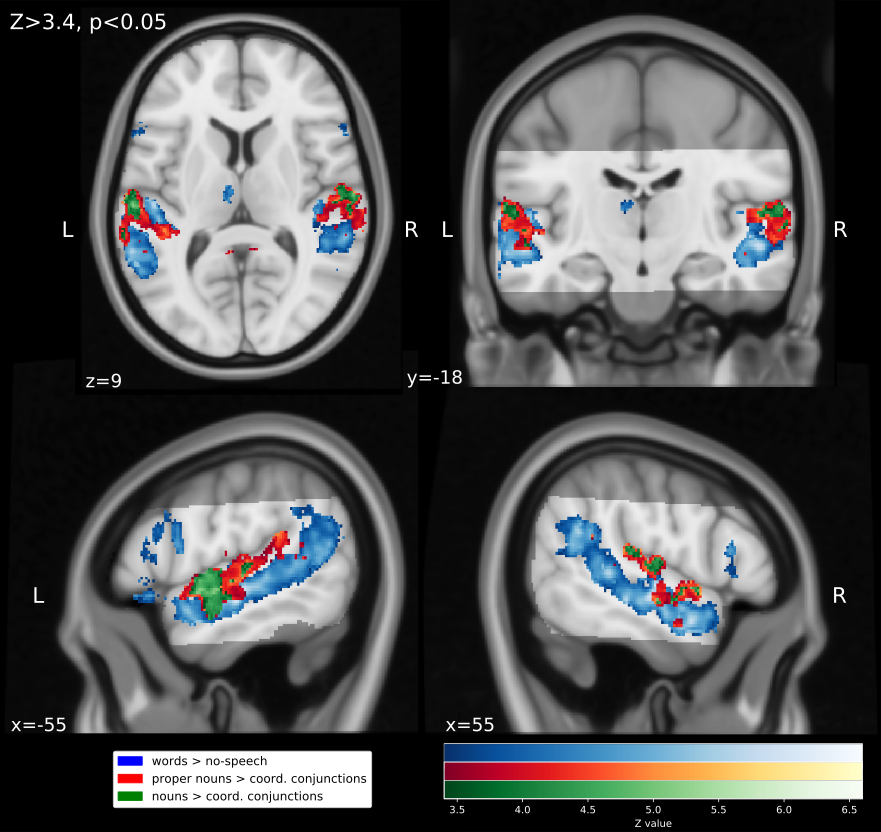
\includegraphics[width=\linewidth]{figures/slicescolorbars}
    \caption{Results of the mixed-effects group-level (N=14) GLM $t$-contrasts
        for the audio-description of the movie ``Forrest Gump''.
        Significant clusters (Z>3.4, p<0.05 cluster-corrected) are overlaid on
        the MNI152 T1-weighted head template (grey).
        Light grey: The audio-description dataset's field-of-view
        (cf. \citep{hanke2014audiomovie}).}
    \label{fig:results}
\end{figure*}


\begin{table*}[t]
\caption{Significant clusters (z-threshold Z>3.4; p<.05 cluster-corrected) for the contrast words (all 21 \texttt{tag}-related regressors) > no-speech.
Clusters sorted by voxel size.
The first brain structure given contains the voxel with the maximum Z-Value,
followed by brain structures from posterior to anterior, and partially covered
areas (l. = left; r. = right; c. = cortex; g. = gyrus).}
\label{tab:cope1}
\begin{tabular}{rrrrrrrrrp{6cm}}
\toprule
& & & \multicolumn{3}{r}{Max location (MNI)} & \multicolumn{3}{r}{Center of gravity (MNI)} &
\\ \cmidrule{4-6} \cmidrule{7-9}
Voxels & $p_{corr.}$ & Z-max & x & y & z  & x & y & z & Structure \\
\midrule
14990 & <.001 & 6.31 & -49 & -24.7 & 6.35 & -54.8 & -32.5 & 3.73 &
l. Heschl's g.;
lateral superior occipital c., angular g., superior \& middle temporal g. (posterior to anterior);
parts of supramarginal g. \& planum temporale \\
14469 & <.001 & 6.48 & 55 & -14.9 & -6.9 & 54.1 & -23.1 & 0.374 &
r. superior temporal g.;
angular g., superior (and middle) temporal g. (posterior to anterior), Heschl's g.;
parts of supramarginal g., planum temporale, pars opercularis (BA44) \& pars triangularis (BA45) \\
1971 & <.001 & 5.26 & -51.1 & 25.6 & -10.5 & -53.6 & 17.8 & 10.2 & l. frontal orbital c.;
pars opercularis (BA44), pars triangularis (BA45);
parts of precentral g. \\
217 & .002 & 4.55 & -4.48 & -13.7 & 10.3 & -6.46 & -14.9 & 9.96 & l. thalamus \\
\bottomrule
\end{tabular}
\end{table*}


\begin{table*}[t]
\caption{Significant clusters (z-threshold Z>3.4; p<.05 cluster-corrected) for the contrast proper nouns (\texttt{ne}) > coordinate conjunctions (\texttt{kon}).
Clusters sorted by voxel size.
The first brain structure given contains the voxel with the maximum Z-Value,
followed by brain structures from posterior to anterior, and partially covered
areas (l. = left; r. = right; c. = cortex; g. = gyrus).}
\label{tab:cope3}
\begin{tabular}{rrrrrrrrrp{6cm}}
\toprule
& & & \multicolumn{3}{r}{Max location (MNI)} & \multicolumn{3}{r}{Center of gravity (MNI)} &
\\ \cmidrule{4-6} \cmidrule{7-9}
Voxels & $p_{corr.}$ & Z-max & x & y & z  & x & y & z & Structure \\
\midrule
7691 & <.001 & 6.23 & -61.2 & -22.3 & 11.6 & -55.9 & -20.7 & 4.03 &
l. planum temporale; posterior inferior supramarginal g., superior temporal g., planum polare,
parts of posterior angular g.,  Heschl's g., middle temporal gyrus \\
5928 & <.001 & 5.5 & 57.5 & -26.2 & 15.9 & 58.2 & -15.8 & 3.55 &
r. planum temporale;
Heschl's g., superior temporal g., planum polare, temporal pole;
parts of angular g. \& posterior inferior supramarginal gyrus \\
479 & <.001 & 4.62 & -5.42 & -32.3 & 25.3 & -4.28 & -39.4 & 22.8 & l. posterior cingulate g. \\
420 & <.001 & 4.85 & -4.76 & -71.4 & 40.1 & -3.74 & -68.5 & 36.2 & l. precuneus \\
407 & <.001 & 5.07 & 6.83 & -40.1 & 24.5 & 6.67 & -38.7 & 23.1 & r. posterior cingulate c. \\
294 & <.001 & 4.57 & 17 & -69.1 & 34.6 & 17.7 & -67.1 & 34.9 & r. precuneus \\
121 & .024 & 3.95 & 8.12 & -98.2 & 0.359 & 8.75 & -97.7 & -3.15 & r. occipital pole \\
117 & .027 & 4.38 & 36.9 & -24.8 & 4.55 & 37.4 & -23 & 3.09 & r. Heschl's g. \\
115 & .029 & 4.08 & -44.6 & -71.7 & 21.7 & -43.6 & -70.8 & 23.4 & l. superior lateral occipital c.\\
\bottomrule
\end{tabular}
\end{table*}


\begin{table*}[t]
\caption{Significant clusters (z-threshold Z>3.4; p<.05 cluster-corrected) for the contrast nouns (\texttt{nn}) > coordinate conjunctions (\texttt{kon}).
Clusters sorted by voxel size.
The first brain structure given contains the voxel with the maximum Z-Value,
followed by brain structures from posterior to anterior, and partially covered
areas (l. = left; r. = right; c. = cortex; g. = gyrus).}
\label{tab:cope5}
\begin{tabular}{rrrrrrrrrp{6cm}}
\toprule
& & & \multicolumn{3}{r}{Max location (MNI)} & \multicolumn{3}{r}{Center of gravity (MNI)} &
\\ \cmidrule{4-6} \cmidrule{7-9}
Voxels & $p_{corr.}$ & Z-max & x & y & z  & x & y & z & Structure \\
\midrule
3166 & <.001 & 5.75 & -61.3 & -10.6 & -2.93 & -57.7 & -14.3 & 1.47 &
l. anterior superior (and middle) temporal g.;
planum temporale, planum polare, anterior superior temporal g.;
part of posterior supramarginal g., Heschl's g. \\
1753 & <.001 & 4.99 & 63.3 & -15.1 & 8.41 & 58 & -13 & 4.02 & r. planum temporale, anterior superior temporal g., planum polare;
part of\& part of Heschl's G. \\
166 & .004 & 4.5 & 6.83 & -40.1 & 24.5 & 7.01 & -39.7 & 24.2 &
r. posterior cingulate g. \\
149 & .008 & 4.13 & 18.2 & -67.8 & 36 & 19.8 & -66.4 & 34.6 &
r. precuneus \\
\bottomrule
\end{tabular}
\end{table*}


% Discussion words > no-speech
For the contrast words > no-speech, results show increased hemodynamic activity
in a bilateral cortical network including temporal, parietal and frontal regions
related to processing spoken language \citep{friederici2011brain,
hickok2007cortical,price2012twentyyears}.
% similarities to previous naturalistic speech paradigms
These clusters resemble results of previous studies that implemented an ISC
approach to analyze fMRI data of naturalistic auditory stimuli
\citep{honey2012not, lerner2011topographic, silbert2014coupled}.
% differences
We do not find significantly increased activations in midline areas (like the
posterior cingulate cortex and precuneus or anterior cingulate cortex and medial
frontal cortex) which showed synchronized activity across subjects in previous
studies.
% Wilson (2008): ISC + GLM
In this regard, our results are similar to \citep{wilson2008beyond} who
implemented both an ISC and a GLM analysis. In this study, the ISC analysis
showed synchronized activity in midline areas but the GLM analysis contrasting
blocks of listening to narratives to blocks of a resting condition showed
significantly decreased activity in these areas.

% (proper) nouns > con
The two contrasts that contrasted nouns and proper nouns respectively to
coordinate junctions yielded increased activation partially located in early
sensory regions (Heschl's Gyrus; \citep{saenz2014tonotopic}) and most
prominently adjacent regions bilaterally (planum temporale; superior temporal
gyrus; \citep{arsenault2015distributed, mesgarani2014phonetic}).
% why these contrasts nous & proper nouns
We chose nouns and proper nouns for these two contrasts because they represent
linguistically similar concepts but are uncorrelated in the German language
and stimulus (cf. Figure \ref{fig:reg-corr}).
% coordinate conjunctions
We contrasted nouns and proper nouns respectively to coordinate conjunctions
because nouns and proper nouns are linguistically different to coordinate
conjunctions as well as uncorrelated.
% “interpretation”
Despite the fact that
nouns and proper nouns are uncorrelated, both contrasts lead to largely
spatially congruent clusters. Results suggest that models based on our
annotation of similar linguistic concepts correlate with hemodynamic activity in
spatially similar areas.
% not driven by coordinate conjunction regressors
We confirmed the validity of these interpretation by testing if the spatial
congruency could be attributed to a negative correlation of coordinate
conjunctions with the modeled time series which turned out not to be the case.
% why it's cool
In summary, results of our exploratory analyses suggest that the annotation of
speech meets basic quality requirements to be a basis for model-based
analyses that investigate language perception under more ecologically valid
conditions.


\section*{Data availability}


\subsection*{Underlying data}

Open Science Framework:
studyforrest-paper-speechannotation.
\href{https://doi.org/10.17605/OSF.IO/GFRME}{https://doi.org/10.17605/OSF.IO/GFRME}.
%Please see email \newline This project contains the following underlying data:
%Please use this section to describe all data files included within your
%dataset. Where there are too many files to describe individually, please
%describe groups of files together.
\begin{itemize}
\item lore ipsum
\end{itemize}


Data are available under the terms of the
\href{https://creativecommons.org/licenses/by/4.0/legalcode}{Creative Commons Attribution 4.0 International license}
% (CC-BY 4.0).

The annotation (tab-separated values (TSV) formatted table and TextGrid file),
as well as scripts and data of the validation analysis are available from
OpenScienceFramework project, and accessible as DataLad (RRID:SCR\_003931)
datasets.%Please confirm - I cannot find this RRID number


\subsection*{Author contributions}
% subsection in Schnitte-Anno
%In order to give appropriate credit to each author of an article, the
%individual contributions of each author to the manuscript should be detailed
%in this section. We recommend using author initials and then stating briefly
%how they contributed.
COH designed, performed, and validated the annotation, and wrote the manuscript.
MH provided critical feedback on the procedure and wrote the manuscript.

\subsection*{Competing interests}
% subsection in Schnitte-Anno
No competing interests were disclosed.

\subsection*{Grant information}
%Please ensure all available grant numbers are provided
COH was supported by a graduate stipend from the German federal state of
Saxony-Anhalt and MH was, in-part, supported by funds from the German federal
state of Saxony-Anhalt and the European Regional Development Fund (ERDF),
Project: Center for Behavioral Brain Sciences (CBBS). Development of the data
management technology used to publish these data on the OpenScienceFramework
was co-funded by the US National Science Foundation (NSF 1912266), and the
German Federal Ministry of Education and Research (BMBF 01GQ1905).


\subsection*{Acknowledgements} COH is grateful to Valeri Kippes who took care
of the author's mental sanity by providing excellent training at his gym in
Jülich during the mentally draining period of manual corrections of the
annotation.
%Please see email
